%%%%%%%%%%%%%%%%%%%%%%% file template.tex %%%%%%%%%%%%%%%%%%%%%%%%%
%
% This is a general template file for the LaTeX package SVJour3
% for Springer journals.          Springer Heidelberg 2010/09/16
%
% Copy it to a new file with a new name and use it as the basis
% for your article. Delete % signs as needed.
%
% This template includes a few options for different layouts and
% content for various journals. Please consult a previous issue of
% your journal as needed.
%
%%%%%%%%%%%%%%%%%%%%%%%%%%%%%%%%%%%%%%%%%%%%%%%%%%%%%%%%%%%%%%%%%%%
%
% First comes an example EPS file -- just ignore it and
% proceed on the \documentclass line
% your LaTeX will extract the file if required
\begin{filecontents*}{example.eps}
%!PS-Adobe-3.0 EPSF-3.0
%%BoundingBox: 19 19 221 221
%%CreationDate: Mon Sep 29 1997
%%Creator: programmed by hand (JK)
%%EndComments
gsave
newpath
  20 20 moveto
  20 220 lineto
  220 220 lineto
  220 20 lineto
closepath
2 setlinewidth
gsave
  .4 setgray fill
grestore
stroke
grestore
\end{filecontents*}
%
\RequirePackage{fix-cm}
%
%\documentclass{svjour3}                     % onecolumn (standard format)
%\documentclass[smallcondensed]{svjour3}     % onecolumn (ditto)
\documentclass[smallextended,envcountsame]{svjour3}       % onecolumn (second format)
%\documentclass[twocolumn]{svjour3}          % twocolumn
%
\smartqed  % flush right qed marks, e.g. at end of proof
%
\usepackage{graphicx}
%
\usepackage{mathptmx}      % use Times fonts if available on your TeX system
%
% insert here the call for the packages your document requires
%\usepackage{latexsym}

\usepackage{amsmath}
\usepackage{amsfonts}
\usepackage{amssymb}
\usepackage{eurosym}
\usepackage{mathtools}
\usepackage{graphicx}
\usepackage{rotating}
\usepackage{setspace}
\usepackage{color}
\usepackage{fancyhdr}
\usepackage{ragged2e}
\usepackage{appendix}
\usepackage{tabularx}
\usepackage{multirow}
\usepackage{booktabs}
\usepackage{xfrac}
\usepackage{pgfplots}
\usepackage{url}
\usepackage{emptypage}
\usepackage{wrapfig}
\usepackage{dsfont}
\usepackage{soul}
\usepackage[dvipsnames]{xcolor}
% \usepackage[backend=bibtex,style=alphabetic]{biblatex}
% \addbibresource{sample.bib}

\usepackage{csquotes}
\usepackage{hyperref}

% \usepackage[
%   backend=biber,
%   style=alphabetic,
%   sorting=nty,
%   maxbibnames=99,
%   url=false,  % Exclude URLs
%   % issn = false
%   %doi=false,   % Exclude DOIs
%   %isbn=false
% ]{biblatex}

% \addbibresource{sample.bib}
%
% please place your own definitions here and don't use \def but
% \newcommand{}{}


\usepackage{xcolor}
\usepackage{todonotes}
\newcommand{\gr}[2][]{\todo[color=violet!40!,#1]{\textsf{GR:} #2}}
\newcommand{\bm}[2][]{\todo[color=blue!20,#1]{\textsf{BM:} #2}}

%\newtheorem{example}{Example}
\newtheorem{assumption}{Assumption}
%\newtheorem{definition}{Definition}
%\newtheorem{theorem}{Theorem}
%\newtheorem{corollary}{Corollary}[theorem]
%\newtheorem{lemma}[theorem]{Lemma}
\newtheorem{prop}[theorem]{Proposition}
\newtheorem{observation}[theorem]{Observation}
%\newtheorem{problem}{Problem}

\DeclareMathOperator{\diag}{diag}
\DeclareMathOperator{\dw}{d_w}
\DeclareMathOperator{\C}{C_{tc}}
\DeclareMathOperator{\T}{T}
\DeclareMathOperator{\MP}{MP}
\DeclareMathOperator{\KP}{KP}
\DeclareMathOperator{\K}{K}
\DeclareMathOperator{\Id}{Id}
\DeclareMathOperator{\SSpan}{Span}
%\DeclareMathOperator{\lim}{lim}
\DeclareMathOperator{\epi}{epi}
\DeclareMathOperator{\supp}{supp}


%\numberwithin{definition}{section}
\numberwithin{theorem}{section}
%\numberwithin{problem}{section}
\newcommand{\nc}{\newcommand}
\nc{\boB}{{\mathbf{B}}}
\nc{\boL}{{\mathbf{L}}}
\nc{\boY}{{\mathbf{Y}}}
\nc{\boI}{{\mathbf{I}}}
\nc{\boV}{{\mathbf{V}}}
\nc{\boS}{{\mathbf{S}}}
\nc{\tV}{{\Tilde{{V}}}}
\nc{\tI}{{\Tilde{{I}}}}
\nc{\tY}{{\Tilde{{Y}}}}
\nc{\tS}{{\Tilde{{S}}}}
\nc{\fr}{{\rightarrow}}
\nc{\co}{{\nabla}}
\nc{\E}{\mathbb{E}}
\nc{\CG}{C_{\Sigma}^{\text{Gauss}}}
\nc{\var}{Var}
\nc{\rows}{S}
\nc{\cols}{R}
\nc{\rowP}{\sigma}
\nc{\colP}{\delta}
\nc{\rowW}{\omega}
\nc{\colW}{\tau}

\nc{\sS}{ \mathscr{S}}
\nc{\sC}{ \mathscr{C}}
\nc{\cH}{{\mathcal H}}
\nc{\cR}{{\mathcal R}}
\nc{\cA}{{\mathcal A}}
\nc{\cG}{{\mathcal G}}
\nc{\cC}{{\mathcal C}}
\nc{\cD}{{\mathcal D}}
\nc{\cO}{{\mathcal O}}
\nc{\cI}{{\mathcal I}}
\nc{\cB}{{\mathcal B}}
\nc{\cY}{{\mathcal Y}}
\nc{\cK}{{\mathcal K}} 
\nc{\cX}{{\mathcal X}}
\nc{\cS}{{\mathcal S}}
\nc{\cE}{{\mathcal E}}
\nc{\cF}{{\mathcal F}}
\nc{\cZ}{{\mathcal Z}}
\nc{\cQ}{{\mathcal Q}}
\nc{\cP}{{\mathcal P}}
\nc{\cL}{{\mathcal L}}
\nc{\cM}{{\mathcal M}}
\nc{\cN}{{\mathcal N}}
\nc{\cT}{{\mathcal T}}
\nc{\cW}{{\mathcal W}}
\nc{\cU}{{\mathcal U}}
\nc{\cJ}{{\mathcal J}}
\nc{\cV}{{\mathcal V}}
\nc{\bH}{{\mathbb H}}
\nc{\bA}{{\mathbb A}}
\nc{\bG}{{\mathbb G}}
\nc{\bC}{{\mathbb C}}
\nc{\bO}{{\mathbb O}}
\nc{\bI}{{\mathbb I}}
\nc{\bB}{{\mathbb B}}
\nc{\bY}{{\mathbb Y}}
\nc{\bK}{{\mathbb K}} 
\nc{\bX}{{\mathbb X}}
\nc{\bS}{{\mathbb S}}
\nc{\bE}{{\mathbb E}}
\nc{\bF}{{\mathbb F}}
\nc{\bZ}{{\mathbb Z}}
\nc{\bQ}{{\mathbb Q}}
\nc{\bN}{{\mathbb N}}
\nc{\bP}{{\mathbb P}}
\nc{\bL}{{\mathbb L}}
\nc{\bM}{{\mathbb M}}
\nc{\bT}{{\mathbb T}}
\nc{\bW}{{\mathbb W}}
\nc{\bU}{{\mathbb U}}
\nc{\bD}{{\mathbb D}}
\nc{\bJ}{{\mathbb J}}
\nc{\bV}{{\mathbb V}}
\nc{\bR}{{\mathbb R}}


\newcommand{\virgolette}[1]{``#1''} %\virgolette{questo č fra virgolette}%
%\usepackage{frontespizio}
\newcommand{\abs}[1]{\lvert#1\rvert}



%
% Insert the name of "your journal" with
\journalname{Optimization and Engineering}
%
\begin{document}

\title{Modelling of a fully renewable energy grid with hydrogen storage: time aggregation for a scalable Capacity Expansion Problem
%\thanks{Grants or other notes
%about the article that should go on the front page should be
%placed here. General acknowledgments should be placed at the end of the article.}
}
\subtitle{}%A stochastic approach considering time interdependence of wind and solar power.}

%\titlerunning{Short form of title}        % if too long for running head

\author{Bianca Urso         \and
        Gabor Riccardi %etc.
}

%\authorrunning{Short form of author list} % if too long for running head

\institute{B. Urso \at
              IUSS School of Advances Studies, Palazzo del Broletto, Piazza della Vittoria, 15 – 27100 Pavia PV, Italy\\
              Tel: +39 0382 375811\\
              Fax: +39 0382 375899\\
              \email{bianca.urso@iusspavia.it}           %  \\
%             \emph{Present address:} of F. Author  %  if needed
           \and
           G. Riccardi \at
           Dipartimento di Matematica ”F. Casorati”
           Via Adolfo Ferrata, 5 – 27100 Pavia
}

\date{Received: date / Accepted: date}
% The correct dates will be entered by the editor


\maketitle

\begin{abstract}
In recent years, the integration of renewable energy sources into electrical grids has become a
critical area of research due to the increasing need for sustainable
and resilient energy systems.  To adress the variability of wind and solar power output over time, electricity grids expansion plans need to account for multiple scenarios over large time horizons.
This significanlty increases the size of the resulting Linear Problem (LP), making them computationally challenging for large scale grids.
To tackle this, we propose an approach that aggregates time steps to reduce the problem size, followed by an iterative refinement of the aggregation. 
\textcolor{violet}{We provide sufficient conditions under which the aggregated problem is equivalent to the original, unaggregated one, and refine the time intervals that do not meet these conditions.
\textbf{write better:Additionally, we introduce a validation function to assess the feasibility of the aggregated solutions. Our method is tested on a fully renewable energy grid with hydrogen storage.}
 We generate scenarios for wind and photovoltaic (PV) power output using scenario generation techniques that capture temporal dependencies. 
 These dependencies are modeled with marginal distributions coupled with a Gaussian copula, ensuring that the generated scenarios reflect realistic 
 temporal correlations observed in historical data.}
%Insert your abstract here. Include keywords, PACS and mathematical
%subject classification numbers as needed.
\keywords{\textcolor{red}{First keyword \and Second keyword \and need 4-6}}
% \PACS{PACS code1 \and PACS code2 \and more}
\subclass{90-10 \and 90B15 }
\end{abstract}

\newpage
\section{INTRODUCTION}

\textbf{Context; literature overview. Small introduction on LP/MIP. Definition of stochastic optimization,
definition of CEP, ED problems.}\\


The threat of climate change is pushing policy-makers to pursue greater integration of renewable energy sources into electrical grids, while at the same time ensuring reliability and resilience through digital optimization of electric power distribution and transmission in smart grids \textcolor{green}{\cite{EU_context}}. One of the main difficulties arising when designing an electric power system relying on renewables is the great variability of the generation of electricity through wind and solar, since these resources are highly dependent on weather conditions, \textcolor{red}{curtailment = inefficient, need hydrogen}, \textcolor{Green}{cite source for hydrogen (eg: EU super investing in it)}. \textcolor{pink}{The stochastic nature of the problem....} making it impossible to plan long-term by optimizing on forecasts, and requiring a statistical approach to ensure a robust model.
Up to now, common approaches have adopted Stochastic Programming (SP) or Robust Optimization (RO) models, along with hybrid models involving Information Gap Decision Theory or Chance Constraint \textcolor{green}{\cite{review_math_opt}}. While initially favored, the SP approach comes with high computational burden, so RO models have seen more popularity in recent years, despite the drawback of being conservative methods with higher average cost of operation and planning of energy systems.\\
\indent In the typical setting, the problem to solve is a Capacity Expansion Problem (CEP) regarding infrastructure investments: solar and wind farms, fuel cells, hydrolizers, grid upgrades to augment Net Transfer Capacity (NTC) and so on. Nested within the CEP is an Economic Dispatch (ED) problem concerning the operational costs of said infrastructure. 
The problem is well suited to be modelled through mixed integer linear programming (MILP), as is explained in detail in \textcolor{green}{\cite{INTRO_isolated_MIP}} and ((\textcolor{Green}{other examples?}))\\
\indent The CEP for investment planning requires to look at long time horizons, and on the other hand intra-day variability in generation \textcolor{pink}{is the main complexity driver} for the ED problem, so the time horizon must be modelled by a large quantity of fairly tight time steps. Furthermore, \textcolor{pink}{spacial structure big, even though we ignore it here and just slam everything into country nodes}. 
Thus the temporal and spacial characteristics of the model bring the MILP size to increase rapidly. This is especially demanding in the case of SP, since all the variables from the inner ED problem must be reproduced over all scenarios.\\
\indent To reduce these costs, one possible approach is to use a Rolling Horizon (RH) \textcolor{red}{[explain better]}. The basic technique is described in \textcolor{green}{\cite{INTRO_Glomb}}, along with some results regarding quality guarantees for the optimality of the solution. In \textcolor{green}{\cite{INTRO_Palma-Behnke}}, a rolling horizon approach is used within a RO model to optimize the operation of a micro-grid composed of \textcolor{pink}{check} serving an isolated area in Chile. \textcolor{Green}{other examples of RH used for the ED} A similar idea is applied in \textcolor{green}{\cite{INTRO_karlsruhe}}, where integer variables representing capital investments are initially relaxed and then progressively fixed in successive time steps, reducing the computational costs associated to the search for integer solutions.\\
\indent A big drawback of the RH approach is that \textcolor{pink}{Problem: it is not optimal. In fact, \cite{INTRO_short-term}. But better reflects actual decision making based on info that is only available progressively, vs perfect foresigh approach.}\\
\indent Our work aims to build a hybrid model, exploring the use of the RH method as a tool to guide progressively tighter relaxations of the perfect foresight model, rather than as a stand-alone technique.  \textcolor{red}{Explain better}. 
Further, RH is then used for the validation of the results for the CEP obtained in the perfect foresight optimization, to ensure that given a solution to the CEP, the ED problem admits feasible solutions even in a limited-foresight environment. The idea is to solve the CEP as to build a grid that can be operated as a "smart grid", \textcolor{pink}{through a control system that optimizes on day ahead forecasts}.\\
\indent The model we optimize on in \textcolor{red}{introduce model: components, aim, use Gurobi...}\\
\indent Finally, to generate the scenarios needed to train and test the SP model, a Gaussian Copula method was used. This has been previously done \textcolor{Green}{here and here and it's not new right?}.\\

This paper is organized as follows: \textcolor{red}{HOW?}\\

%\textbf{OLD:}
%\textcolor{gray}{
%The threat of climate change is pushing policy-makers to pursue greater integration of renewable energy sources into electrical grids, while at the same time ensuring reliability and resilience of the grids \cite{EU_context}. The model presented in this report explores the possibility of an electrical grid powered entirely through wind and photovoltaic (PV) systems, and supported by hydrogen storage.
%It is of interest to estimate the power generation capacity for both wind and solar, as well as the hydrogen storage and conversion capacities, that would be necessary in order to power a reliable grid supplying residential electricity load and industrial base load of both electricity and hydrogen for a given area, while minimizing the cost of implementing such infrastructure.
%The main difficulties arising when designing such a system lie in the great variability of the generation of electricity through wind and solar, since these resources are highly dependent on weather conditions, making it impossible to plan long-term by optimizing on forecasts, and requiring a statistical approach to ensure a robust model.
%The scenario generation step is followed by an optimization process. The model, as described in section \ref{section: model}, takes in input the generation and load scenarios of the selected countries along with various parameters indicating costs and efficiency of the current state of technology and possible upper bounds for the decision variables, and returns the optimized capacity that is necessary to meet demand throughout a one year span, with minimal cost. The optimization problem is solved using the Gurobi solver.
%When optimizing over multiple scenarios jointly, the solver returns the minimal amount of infrastructure and capacities that is needed to have feasibility (that is, demand met at all time - no blackouts) over all scenarios in input, with minimal average cost over the scenarios.
%When considering a network with more than a single node, computational costs increase rapidly. Thus a small analysis is carried out to determine acceptable time steps on which time dependent data can be aggregated (the gathered data is usually on hourly steps) while maintaining the quality of the solution. 
%Results are then evaluated for a single node network and for more complex networks based in the European Union, for which the necessary data was publicly available. Appropriate validation functions are discussed to check feasibility over new scenarios, along with cost functions that give more realistic cost estimates compared to the optimal value given by the solver.
%}




\section{MODEL}

\subsection{LP Formulation}\label{section: LP}
Our model describes a network in Europe that is to be powered and supplied of hydrogen trough power generated by photovoltaic panels and wind turbines, converted to hydrogen through electrolysis and potentially reconverted in fuel cells.


The network is represented by an undirected multigraph \(\cG = (\cN, \cE)\), where \(\cN\) corresponds to the nodes in the network, and \(\cE = \cE_H \cup \cE_P\) represents transmission lines (\(e \in \cE_P\)) and hydrogen lines (\(e \in \cE_H\)). Each of these nodes can be in different countries in Europe, and the power generated by wind and solar power depends on the node location. In particular, if node \(n \in \cN\) is in France, the scenarios for power generation at \(n\) will be generated using parameters fitted to France's data.

Each node has its generators, hydrogen storage, fuel cells and hydrolyzers, for which the capacity is to be decided. Likewise, the CEP aims to solve for transmission line NTC and hydrogen pipe transmission capacity for each edge of the network. The basic formulation of the LP \textcolor{pink}{described in this section} allows us to solve the CEP with perfect foresight. \\
\indent We decided to model our problem as a LP problem instead of MILP, as would be standard in the literature \textcolor{Green}{SOURCES?}. This is because when modelling a large grid with high demand, optimizing on continuous variables and then rounding up to the closest integer for variables $ns$ and $nw$ notably decreases computational costs, without relevant difference in the final cost. The same wouldn't be possible when optimizing over micro-grids.\\
\indent The model takes in input the generation and load scenarios of the given area along with various parameters indicating costs and efficiency of the current state of technology and possible upper bounds for the decision variables. The CEP and the ED problems for all scenarios are solved concurrently. When optimizing over multiple scenarios jointly, the solver returns the minimal amount of infrastructure and capacities that is needed to have feasibility (that is, demand met at all time and no blackouts) over all scenarios in input, with minimal cost. Cost is considered to be the sum of capital costs and average operational costs of the infrastructure over the scenarios.\\
\indent The optimization problem is solved using the Gurobi solver \textcolor{green}{\cite{Gurobi}}.



%%%%%%%%%%%%%%%%%%%%%%%%%%%%%%%  VARIABLES  %%%%%%%%%%%%%%%%%%%%%%%%%%%%%%%%%%%%%

\subsubsection{Decision Variables}

The main variables that are of interest to the policy maker are, for each location $n$, the number of wind turbines and PV panels to install, as well as hydrogen storage capacity.
Stored hydrogen is considered to be the total of liquid and gas hydrogen to be stored. Our model does not assume a distinction between the two forms, and considers hydrogen to be immediately ready for long-term storage as soon as it is converted from electricity, as well as instantaneously convertible to electricity in fuel cells at need. \textcolor{Green}{For more detailed models of the management of hydrogen see SOURCES}.\\
\indent Important values to consider when planning the grid are the power capacity and conversion speed of fuel cells and electrolyzers: variables $mhte_n$ and  $meth_n$ indicate for each location the maximum amount of energy that can be converted at a single time step respectively from hydrogen to electricity and vice versa. These values are essential to estimate in order to design a grid that can effectively accommodate peak production and supply during low production periods.\\
\indent \textcolor{Green}{explain what NTC is? quote paper.} Existing NTC is estimated through the procedure followed by \hyperlink{https://www.diva-portal.org/smash/get/diva2:1476768/FULLTEXT01.pdf}{link} \textcolor{pink}{(page 30)}, by collecting data from \hyperlink{https://transparency.entsoe.eu/transmission-domain/physicalFlow/show?name=&defaultValue=false&viewType=TABLE&areaType=BORDER_CTY&atch=false&dateTime.dateTime=22.07.2024+00:00|CET|DAY&border.values=CTY|10YGR-HTSO-----Y!CTY_CTY|10YGR-HTSO-----Y_CTY_CTY|10YIT-GRTN-----B&dateTime.timezone=CET_CEST&dateTime.timezone_input=CET+(UTC+1)+/+CEST+(UTC+2)}{link}. Improvements on the existing capacity for power lines or hydrogen transport infrastructure are considered through variables $addNTC_l$ and $addMH_l$. \textcolor{Green}{cite EU policy to upgrade grid}.\\
\indent Variables linked to the inner ED problem are indexed by scenario \(j\), time step \(t\), and either node \(n \in \cN\)  or edge $l\in\cE_H$ or $l \in \cE_P$. For the variables pertaining to transmission on an edge, two distinct variables are considered, one for each direction. This way, all variables are set to be non-negative. \textcolor{pink}{This will be relevant for the formulation of the time-aggregated relaxation of the LP problem.}\\

See Table \ref{table_vars} for the summary of all decision variables.


% For tables use
\begin{table}
  % table caption is above the table
  \caption{Decision variables}
  \label{table_vars}       % Give a unique label
  % For LaTeX tables use
  \begin{tabularx}{\textwidth}{ccl}
  \hline\noalign{\smallskip}
  \textbf{Name} & \textbf{Unit} & \textbf{Description}  \\
  \noalign{\smallskip}\hline\noalign{\smallskip}
  $\text{ns}_n$ & - & Number of solar units at node $n \in \cN$ \\
  $\text{nw}_n$ & - & Number of wind units at node $n \in \cN$ \\
  $\text{nh}_n$ & kg & Storage capacity at node $n \in \cN$\\
  $\text{mhte}_n$ & kg & \parbox[t]{0.70\textwidth}{Maximum hydrogen to electricity capacity,  at node $n \in \cN$} \\
  $\text{meth}_n$ & MWh & Maximum electricity to hydrogen capacity at node $n \in \cN$\\
  $\text{addNTC}_l$ & MWh & Additional net transfer capacity on line $l$;\\
  $\text{addMH}_l$ & kg & Additional hydrogen transfer capacity on pipe $l$\\
  \noalign{\smallskip}\hline\noalign{\smallskip}
  $\text{H}_{j,t,n}$ & kg& Stored hydrogen at node $n$, time \(t\), scenario \(j\)\\
  $\text{HtE}_{j,t,n}$ & kg& Hydrogen converted to electricity at time \(t\),scenario \(j\) \\
  $\text{EtH}_{j,t,n}$ & MWh& Electricity converted to hydrogen at time \(t\), scenario \(j\)\\
  P\_edge$^+_{j,t,l}$&MWh& Power passing through line $l$ at time $t$, scenario $j$ \\
  P\_edge$^-_{j,t,l}$&MWh& Power passing through line $l$ at time $t$, scenario $j$ \\
  H\_edge$^+_{j,t,l}$&kg& Hydrogen transported through line $l$ at time $t$, scenario $j$\\
  H\_edge$^-_{j,t,l}$&kg& Hydrogen transported through line $l$ at time $t$, scenario $j$\\
  \noalign{\smallskip}\hline
  \end{tabularx}
  \end{table}
  


%%%%%%%%%%%%%%%%%%%%%%%%%%%%%%%  PARAMETERS  %%%%%%%%%%%%%%%%%%%%%%%%%%%%%%%%%%%%%

\subsubsection{Parameters}

\indent There are a series of parameters that describe the grid and are passed to the model. The main ones are related to capital costs of the infrastructure to be built and the following values are assumed for panels and turbines: $cs = 400$\euro, $cw = 3 000 000$\euro. 
We also set capital costs for fuel cells and electrolyzers. tjese can be set to minimal "symbolic" costs just to ask the solver to estimate needed capacity, so that they are minimized through the model, or they can be set to actual investment for the facilities. Since hydrogen infrastructure is usually obtained by reconverting existing infrastructure from other purposes, the estimation of investment costs is very location dependent and beyond the scope of this work. Thus for our purposes, a symbolic minimal cost was used. \textcolor{Green}{cite article}.\\
\indent The storage of the hydrogen has a cost that depends on various factors: capital cost of the technology used for storage, operating costs, length of time that the hydrogen is kept in storage. For our model we only set the parameters $ch$, to be multiplied by the maximum storage needed ($nh$), representing capital cost of storage infrastructure. We ignore marginal costs of keeping the hydrogen stored. \\

\indent In this model we assume no marginal costs for PV and wind power production: the operating costs of the farms throughout their life-cycle can be factored into the capital costs, and there is no additional cost linked to the production itself. \\
\indent Conversely, the marginal costs of conversion within electrolyzers and power cells are relevant. According to the European Hydrogen Market Landcape November 2023 Report  \textcolor{green}{\cite{European_H2_Market_landscape}}, ``Hydrogen production costs via electrolysis with a direct connection to a renewable energy source in Europe vary from 4.18 to 9.60 €/kg H2 of hydrogen, with the average for all countries being 6.86 €/kg H2''. For electrolyzers, we consider the Levelised cost of hydrogen (LCOH)  to account for both marginal costs and capital costs. Such cost is dependent on the country's specific market condition and can be calculated through the \textcolor{green}{\href{https://observatory.clean-hydrogen.europa.eu/tools-reports/levelised-cost-hydrogen-calculator}{European Hydrogen Observator tool}}.\\
\indent Parameters $fhte_n$ and $feth_n$ are set as scalars between $0$ and $1$ to indicate efficiency of the conversion from hydrogen to electricity and vice versa. It is assumed that 1kg of hydrogen has an energy value of 33kWh \textcolor{green}{cite}. Thus if we consider an electrolyzer operating at maximum efficiency ($feth=1$), one MWh of electricity yields 1000/33$\simeq$30kg of hydrogen. For our purposes, a standard value of $feth=0.66$ is considered, thus 1MWh yields 20kg of hydrogen. Conversely, in a fuel cell operating at maximum efficiency ($fhte=1$) 1kg of hydrogen yields 33kWh. We consider a value of $fhte=0.75$, yielding 24.75kWh per kg of hydrogen. Actual efficiencies vary a lot depending on the technology used. Furthermore, chemical and physical constraints make it so that efficiencies higher than 0.80-0.85 are currently considered unachievable \cite{DAWOOD}.\\
\indent Additionally, we assume the flow of electricity has no marginal cost nor power loss (the modelling of that problem is beyond the scope of this project), whereas we do set a cost for the use of hydrogen pipes (or other means of transfer). The existing capacity of transmission lines and hydrogen pipes is also set. \textcolor{green}{mention again the same as before?}\\
\indent Finally, the model allows for upper bounds to be placed on the variables, based on either technological and physical constraints (dimension of the facilities) or because of political choices (e.g. local population unfavourable to wind turbines).\\

\indent The parameters $ES, EW, EL, HL$, indexed by scenario, time step and node represent the time series of power generation and load values for different scenarios in every node of the grid. They are generated through the method described in \textcolor{pink}{the appendix \ref{generation}}\\

\indent See Table \ref{table_param} for the summary of all parameters. 

% For tables use
\begin{table}
  % table caption is above the table
\caption{Model parameters}
  \label{table_param}       % Give a unique label
  % For LaTeX tables use
\begin{tabularx}{\textwidth}{ccl}
  \hline\noalign{\smallskip}
    \textbf{Name} & \textbf{Unit} & \textbf{Description}  \\
  \noalign{\smallskip}\hline\noalign{\smallskip}
    cs & \euro& Cost of one Solar Panel at node $n$\\
    cw & \euro & Cost of one Wind Turbine at node $n$\\
    chte$_n$ & \euro/kg & Conversion cost of \textcolor{Cerulean}{$H_2$} to electricity \\
    ceth$_n$ & \euro/MWh & Conversion cost of electricity to hydrogen \\
    ch$_n$ & \euro/kg & Cost of hydrogen storage capacity\\
    cH\_edge$_l$ & \euro & Cost of transferring 1kg of hydrogen through edge $l$\\
    cNTC$_l$ & \euro/MWh & Cost of adding NTC to line $l\in\cE_P$\\
    cMH$_l$ &\euro/kg& Cost of adding $H_2$ transfer capacity to line $l\in\cE_H$\\
    \textcolor{pink}{cmhte} &&\\
    cmeth &&\\
  \noalign{\smallskip}\hline\noalign{\smallskip}
    fhte$_n$ & - & Efficiency of hydrogen to electricity conversion \\ 
    feth$_n$ & - & Efficiency of electricity to hydrogen conversion \\
    NTC$_l$ & MWh & Net Transfer Capacity on line $l\in\cE_P$\\
    MH$_l$ & kg &  Hydrogen transfer capacity on edge \textcolor{Cerulean}{$l\in\cE_H$}.\\
  \noalign{\smallskip}\hline\noalign{\smallskip}
    Mns$_n$ & - & Maximum number of solar panels installable at node $n$\\ 
    Mnw$_n$ & - & Maximum number of wind turbines that can be installed \\ 
    Mnh$_n$ & kg & Maximum hydrogen storage capacity \\
    Mhte$_n$ & kg & Upper bound for \textcolor{Cerulean}{\(mhte\)} \\ 
    Meth$_n$ & MWh & Upper bound for \(meth\) \\
  \noalign{\smallskip}\hline\noalign{\smallskip}
    ES$_{j,t,n}$ & MWh & Power output of a single solar panel\\
    EW$_{j,t,n}$ & MWh & Power output of a single wind turbine \\
    EL$_{j,t,n}$ & MWh & Electricity load \\
    HL$_{j,t,n}$ & kg & Hydrogen load\\
    \noalign{\smallskip}\hline
\end{tabularx}
\end{table}


%%%%%%%%%%%%%%%%%%%%%%%%%%  OBJECTIVE FUNCTION  %%%%%%%%%%%%%%%%%%%%%%%%%%%%%

\subsubsection{Objective Function}
The cost function is given by the sum of all capital costs of installing infrastructure, plus all marginal costs of the hydrogen to electricity and electricity to hydrogen conversions and hydrogen transfer on the edges at each time step
% \begin{align*}
%     \min \quad & \text{cs} \cdot \text{ns} + \text{cw} \cdot \text{nw} + \text{ch} \cdot \text{nh} + \\
%     & + \frac{1}{d}\sum_{j=1}^{d} \sum_{i=1}^{\text{inst}} (\text{ch\_t} \cdot \text{H}_{j,t} + \text{chte} \cdot \text{HtE}_{j,t} + \text{ceth} \cdot \text{EtH}_{j,t}) +\\
%     & + 0.01*(mhte + meth).
% \end{align*}
Let $Nnodes$, $NPedges$ and $NHedges$ be the number of nodes, edges on the electric grid graph and edges of the hydrogen transfer graph respectively. Let $d$ be the number of scenarios, and $T$ the number of time steps. The objective function is as follows:
\begin{align*}
    \min \quad 
    &&\sum_{k\in\cN}&(\text{cs}_k \cdot \text{ns}_k+\hspace{-1em}&&\text{cw}_k \cdot \text{nw}_k + \text{ch}_k \cdot \text{nh}_k )\ + \\
    &+& \sum_{k\in\cN}&(\text{cmhte}_k\cdot\text{m} \hspace{-2em}&& \text{hte}_k + \text{cmeth}_k\cdot \text{meth}_k) \ + \\
    &+& \sum_{l\in\cE_P}& (\text{cNTC}_l\cdot \text{ad}\hspace{-2em}&&\text{dNTC}_l) 
    + \sum_{l\in\cE_H} (\text{cMH}_l\cdot \text{addMH}_l) \ + \stepcounter{equation}\tag{\theequation}\label{objVal} \\   
    &+&\frac{1}{d}\sum_{j=1}^{d}&\sum_{t=1}^{T} \Bigg(\sum_{k\in\cN} \hspace{-5em}&&
    (\text{ch\_t}_k \cdot \text{H}_{j,t,k} + \text{chte}_k \cdot \text{HtE}_{j,t,k} + \text{ceth}_k \cdot \text{EtH}_{j,t,k})\ + \\
    &&&\hspace{-2em}&&+\sum_{l\in\cE_H} (\text{cH\_edge}_l\cdot\text{H\_edge}_{j,t,l}) \Bigg)
\end{align*}

The $1/d$ factor in front of the marginal costs allows to average over the scenarios, whereas the capital costs are the same for all scenarios. Thus, ignoring the costs of $mhte_k$ and $meth_k$, the objective function value gives an estimate of the actual costs (in \euro) for the set up and maintenance of the system throughout the length of the time horizon. 


%%%%%%%%%%%%%%%%%%%%%%%%%%%%%%%  CONSTRAINTS  %%%%%%%%%%%%%%%%%%%%%%%%%%%%%%%%%%%%%

\subsubsection{Constraints}
The following constraints are to ensure that for all time steps $t$ and all scenarios $j$, the electricity load and the hydrogen load are met. The measure units are MWh and kg respectively, and conversion factors are considered for $HtE$ and $EtH$ respecively.
Let $Out(n)$ and $In(n)$ indicate the outgoing and incoming edges from node $n$ on the respective graph. For simplicity, we indicate with $P\_edge_{j,t,l}$ the difference of the corresponding variables $P\_edge^+_{j,t,l}-P\_edge^-_{j,t,l}$, and analogously for $H\_edge$. When solving, it is sufficient to assign a symbolic cost to them to ensure that only one of them is non zero at each time step. Then for each node $n$, the following flow balance constraints are imposed:
\begin{align*}
    \text{Electricity Balance:} \quad & \text{ns}_n \cdot \text{ES}\hspace{-1.2em}&_{j,t,n}&+ \text{nw}_k \cdot \text{EW}_{j,t,n} - \text{EL}_{j,t,n} \ + \\
    &  + 0.033\hspace{-2em}& \cdot f&hte_k \cdot \text{HtE}_{j,t,n} - \text{EtH}_{j,t,n}\ + \stepcounter{equation}\tag{\theequation}\label{constr_P}\\
    & + \sum_{l\in Out(n)}\hspace{-1.9em}&\text{P\_}&\text{edge}_{j,t,l} + \sum_{l\in In(n)} \text{P\_edge}_{j,t,l} \ge 0;\\
    \text{Hydrogen Storage:} \quad & \text{H}_{j,t+1,n} \hspace{-5em}&=& \text{H}_{j,t,n} - \text{HL}_{j,t,n}\ +\\ 
    &&& + 30 \cdot feth_k \cdot \text{EtH}_{j,t,n} - \text{HtE}_{j,t,n} \ + \stepcounter{equation}\tag{\theequation}\label{constr_H}\\
    &&& - \sum_{l\in Out(n)}\text{H\_edge}_{j,t,l} + \sum_{l\in In(n)}\text{H\_edge}_{j,t,l}
\end{align*}

We ask that the consumed electricity be less or equal than the produced or received electricity at all times. On the grid itself, the two sides should be equal, but we observe that $ns\cdot ES_{j,t} + nw\cdot EW_{j,t}$ indicate the maximum power that can be generated with set weather conditions, whereas actual production will be regulated to meet demand through curtailment. \textcolor{pink}{if set to =, see paper??}

The stored hydrogen at time $t+1$ is the result of what was stored at time $t$ adjusted by what was converted and what was sent to the industrial load. For $t=T$ (the last time step) we set the same constraint on hydrogen by considering $t+1$ to be index $1$: this way we avoid placing a ``start time'' at an arbitrary place within the year (time is rendered modulo the year) and we avoid the model asking for conveniently high initial storage values of hydrogen appearing out of thin air.

The total storage and conversion capacities are calculated by minimizing the maximum over time and scenarios of the variables $H_{j,t}, EtH_{j,t}$ and $HtE_{j,t}$, for all scenarios \(j\), time steps \(t\) and nodes \(n\):

\begin{align*}
    \text{Storage Capacity Limit:} \quad & \text{H}_{j,t,n} \leq \text{nh}_n ;\stepcounter{equation}\tag{\theequation}\label{constr_nh}\\
    \text{EtH Conversion Limit:} \quad & \text{EtH}_{j,t,n} \leq \text{meth}_n; \stepcounter{equation}\tag{\theequation}\label{myeq1}\\
    \text{HtE Conversion Limit:} \quad & \text{HtE}_{j,t,n} \leq \text{mhte}_n .\stepcounter{equation}\tag{\theequation}\label{myeq1}
\end{align*}
Finally, edge capacities on the respective graphs are considered for all scenarios \(j\), time steps \(t\) and nodes \(n\):
\begin{align*}
    \text{Net Transfer Capacity:} \quad & \text{P\_edge}^\pm_{j,t,l}\le\text{NTC}_l + \text{addNTC}_l ;\stepcounter{equation}\tag{\theequation}\label{myeq1}\\
    \text{Hydrogen Transfer Capacity:} \quad & \text{H\_edge}^\pm_{j,t,l}\le\text{MH}_l + \text{addMH}_l.\stepcounter{equation}\tag{\theequation}\label{myeq1}
\end{align*}




%%%%%%%%%%%%%%%%%%%%%%%%%%%%%%%%%%%%%%%%%%%%%%%%%%%%%%%%%%%%%%%%%%%%%%%%%%%%%%%%%%%%%%%%%%%%%%%%%%%%%%%
%%%%%%%%%%%%%%%%%%%%%%%%%%%%%%%%%%%%%%%%%%%%%%%%%%%%%%%%%%%%%%%%%%%%%%%%%%%%%%%%%%%%%%%%%%%%%



\subsection{Validation: Rolling Horizon}

While computing the optimal solution on a batch of scenarios by solving the LP model described in \textcolor{pink}{section} \ref{section: LP}, the solver ``knows the future'' for those scenarios. That is, the criteria it uses to determine, at each time step, how much electricity or hydrogen should be converted or transmitted, and where, is a mathematical minimum that is informed by the knowledge of what is needed at any time during the one year scenario.
In real life, accurate forecasts for weather, and consequently for power generation, are known on a day ahead basis, at most two days ahead. We are thus interested in evaluating whether an optimal grid as given by the solution of the CEP problem on a batch of train scenarios can (1) be operated without knowledge of the future in order to satisfy demand on the same scenarios it was trained on, and (2) generalize to new test scenarios.\\

\indent Let's first consider the case where the grid is composed of a single node. The actions and choices of a power grid administrator of such an isolated micro-grid are very much limited to ``given extra energy, store it, up to storage limit''. Such a strategy is for example discussed in more detail in \textcolor{green}{\cite{deterministic}}. A deterministic system control can be easily designed to check whether a single node CEP solution is sufficient for feasibility over a certain scenario, even without day ahead forecasts.
This is not true anymore once the node is taken out of isolation: at each moment, without knowledge of the full future, each fictional administrator at each node must choose whether to store the energy generated at their node, whether to send it to a neighbor (and how much to which neighbor) or how to collect missing energy to match their node's demand.\\

\indent In order to operate a multi-node grid, we propose to use the Rolling Horizon optimization technique. 
The basic idea, as described in \textcolor{green}{source} is to divide the time horizon into smaller periods and to progressively optimize on each period, passing the variables of the solved periods as fixed to the next. In our case, we are interested in periods of length one day each, representing the knowledge of future that is given to the grid administrator by weather forecasts.  \\

Recall that when optimizing with the LP model described in \textcolor{pink}{section \ref{section: LP}}, the solutions to the CEP and to the ED problem for all train scenarios $j\in J_{train}$ are given concurrently. Consider now a test scenario with generation and load time series $ES_{t,n}, EW_{t,n},$ $EL_{t,n}, HL_{t,n}$ (the test scenario can be in $J_{train}$ or not).
\color{red}
\begin{itemize}
\item start with $H_{0,n} = \max_{j\in J_{train}} H_{j,0,n}$\\
\item for each day in the time horizon, optimize the inner ED problem for that day
\item set the hydrogen storage levels of the last time step of the day equal to the ones for the first time step of the next day.

\end{itemize}\color{black}

The daily ED problem is formulated in a similar way to the LP problem described in section \ref{section: LP}. The differences are that the CEP variables ($ns$, $nh$,...) are fixed, and the hydrogen storage level doesn't loop as it did in the year, but it connects to the following day. \\

\begin{definition}[RH-feasibility]
  Given a solution $x_{CEP}$ to the CEP solved over train scenarios $j\in J_{train}$ and a test scenario $j$, we consider $x_{CEP}$ to be RH-feasible over scenario $j$ if the RH optimization algorithms terminates at the end of the year and $H_{j,T,n}\ge H_{j,0,n}$ for all nodes $n\in\cN$.
  \end{definition}
  We require the last condition to mean that the storage levels at the end of the year are at least as high as they were at the start, to flag as unfeasible solutions that satisfy demand throughout the year with a net consumption of unproduced hydrogen.\\
  

Written as such, the daily optimization would tend to avoid storing hydrogen unless needed within the same day, since operating the elecrolyzers has a cost. This easily renders infeasible scenarios that would be feasible with better storage management. 
To solve this problem, one can introduce a loss function in the model: for example one can assign a cost to the difference between the hydrogen storage level at time step $t$ and the average over the corresponding variables in the optimal solutions from train scenarios. Thus one defines positive variables $loss_{t,n}$ for each time step $t$ and node $n$, with posiitive cost, and adds the contraint:
\begin{equation}
loss_{t,n} \ge \frac{1}{d}\sum_{j\in J_{train}} H_{j,t,n} - H^{test}_{t,n} 
\end{equation}
Another option would be to assign a slight negative cost to $H^{test}_{t,n}$, to incentivize filling up the storage, but this can inflate the estimated cost of operating electrolyzers more than necessary.\\


We observe that the overall solution to the ED problem throughout the full time horizon obtained by means of the RH method is not necessarily optimal, neither with nor without the added loss function. However, some results can be obtained regarding the distance of such solution from the optimal of the ED problem. Indeed:
\textcolor{red}{The first step ensures that conditions 1-4 from \textcolor{green}{cite paper} are satisfied. Thus we have near optimality guarantee....}\\
%On the other hand, we observe that no information is given on whether the CEP solution is optimal on the test scenario: we can only evaluate feasibility. For  
For a solution to the ED problem that is closer still to the perfect foresight optimal, more refined RH tecniques can be used. For example, optimizing on two-day forecasts with a daily refresh rate, as done in \textcolor{green}{source} can improve the quality of the solution. However, for our purposes, being able to check for feasibility with less than optimal management is sufficient.




%%%%%%%%%%%%%%%%%%%%%%%%%%%%%%%%%%%%%%%%%%%%%%%%%%%%%%%%%%%%%%%%%%%%%%%%%%%%%%%%%%%%%%%%%%%%%%%%%%%%%%%
%%%%%%%%%%%%%%%%%%%%%%%%%%%%%%%%%%%%%%%%%%%%%%%%%%%%%%%%%%%%%%%%%%%%%%%%%%%%%%%%%%%%%%%%%%%%%



\section{Time Resolution}\label{section:time-resolution}


The scenarios generated from our gathered data have a time resolution of one hour. \textcolor{red}{where have I said this for the first time?}. Such resolution is enough to capture the daily variability of power generation and load. However, the number of variables and constraints grows linearly with the number of time steps, making the model intractable with just a few scenarios.
Moreover, when optimizing over a full year, considering every hour of every day is partly redundant, as each day will be similar to neighboring days. Yet, simply considering a sample of days for each season might undermine long-term storage capacity representation. Thus we are interested in finding more efficient ways to deal with the time dimension in our problem. \\

\subsection{Time aggregation as model relaxation}
We introduce the following concept:

\begin{definition}
Given an initial time horizon \(\cT = \{1, \ldots, T\}\), a time partition  \(P=\{I_1,...,I_{T'}\}\) is a partition of \(\cT\) such that all subsets are intervals. Furthermore, we say that a time partition \(P'\) is finer than \(P\) if for every \(I' \in P'\), there exists some \(I \in P\) such that \(I' \subset I\).
\end{definition}

Given a time partition $P$, we can consider the problem \(CEP_P\) associated to the model obtained by considering each interval in \(P\) as a single time step. For every \(I\in P\), define:
\[
ES_{j,I,n} \coloneqq \sum_{i \in I} ES_{j,i,n}, \quad\quad EW_{j,I,n} \coloneqq \sum_{i \in I} EW_{j,i,n}, 
\]
and analogously for $EL_{j,I,n}$ and $HL_{j,i,n}$. \\

It is easy to show that the optimal value to the aggregated problem \(CEP_P\) is a lower bound for the original problem \(CEP_{\cT}\). Indeed, given a feasible solution of the latter, we can obtain a solution of the former by fixing the capital infrastructure variables to be the same as in \(CEP_{\cT}\) and letting all time dependent variables for the inner ED problems be defined as follows:
\[
EtH_{j,I,n} = \sum_{i \in I} EtH_{j,i,e}, \quad\quad HtE_{j,I,e} = \sum_{i \in I} HtE_{j,i,e},  \quad\quad \Delta H_{j,I,e} = \sum_{i \in I} \Delta H_{j,i,e};
\]
similarly, we sum over \(P\_edge^\pm_{j,I,e}\) and \(H\_edge^\pm_{j,I,e}\), separately on the two directions.
By defining the aggregated variables this way, the aggregated constraints are not violated, thus we get a feasible solution to \(CEP_P\).
Observe that all variables with non zero cost are defined as greater or equal to zero, so summing over them we define a cost-preserving linear map from the solution space of \(CEP_{\cT}\) to the solution space of \(CEP_P\).\\

The above discussion holds in general in the case of any two partitions $P$ and $P'$ where $P'$ is finer than $P$.
We can summarize the above in the following observation:
\color{pink}
\begin{observation}
Let $P$ and $P'$ be two time partitions of $\cT=\{1...T\}$ such that $P'$ is finer than $P$. Let \(V_{P} \subset \bR^{N_{P}}\) and \(V_{P'} \subset \bR^{N_{P'}}\) be the spaces of feasible solutions of \(CEP_{P}\) and \(CEP_{P'}\), respectively. Then there exists a linear map \(L: \bR^{N_{P'}} \to \bR^{N_{P}}\) such that \(L(V_{P'}) \subset V_{P}\) and \(c_{P}(L(x)) = c_{P'}(x)\), where \(c_{P}\) is the cost function of \(CEP_{P}\) and \(c_{P'}\) is the cost function of \(CEP_{P'}\).
Then the optimal solution to $CEP_{P}$ provides a lower bound for $CEP_{P'}$
\end{observation}
\color{black}


\textcolor{red}{To clarify what time aggregation implies on the model constraints, we express the LP problem in matrix form, in order to highlight its inner structure.}
%Varying time aggregation can be viewed as performing row and column aggregation on the original linear programming (LP) model. Consider the following general linear problem:
The goal is to write our problem in standard form:
\begin{align*}
\min_{x \in \bR^{n}} &c^T x \\ 
\text{s.t.} &\quad Ax = b \stepcounter{equation}\tag{\theequation}\label{std_LP}\\
&x \geq 0
\end{align*}

Fistly, we can reformulate the model described in \ref{section: LP} by introducing a new set of variables 
\(h_{j,t,n} \coloneqq H_{j,t+1,n} - H_{j,t,n}\), replacing the original variables \(H_{j,t,n}\). Constraints (\ref{constr_H}) and (\ref{constr_nh}) shall be reformulated accordingly, with the latter becoming:

\begin{align}
  \sum_{i=1}^{t} h_{i,j,n} \le nh_{n}, & \quad \forall\  t =1...T, \tag{\ref{constr_nh}$'$}\label{eq:delta_hydrogen_constraints}
\end{align}

%Here, \(A\) is an \(m \times n\) matrix. Now, let \(\rowP = \{\rows_1, \rows_2, \ldots, \rows_{\tilde{n}}\}\) be a partition of \([n]\) (the columns) and \(\colP = \{\cols_1, \cols_2, \ldots, \cols_{\tilde{m}}\}\) a partition of \([m]\) (the rows), corresponding to a partition of the rows and columns of \(A\).

%We obtain the corresponding aggregated problem by replacing each set \(\rows\) in \(\rowP\) with a single row, and each set \(R\) in \(\colP\) with a single column. 
%One way to aggregate a set of rows (or columns) is by taking a linear combination of the rows (or columns), known as \emph{weighted aggregation}.
%We denote the coefficients of the aggregation by \(\rowW_r\) for \(r \in \rowP\), and \(\colW_c\) for \(c \in \colP\).
%The corresponding aggregated LP problem becomes:
%\begin{align}
%\label{eq:LPaggr}
%\min_{\tilde{x} \in \bR^{\tilde{n}}} &\tilde{c}^T \tilde{x} \\ 
%\text{s.t.} &\quad \tilde{A} \tilde{x} = \tilde{b} \\ 
%&\tilde{x} \geq 0 
%\end{align}
%where \(\tilde{A}\) is a \(\tilde{m}\times \tilde{n}\) matrix.

In the problem under consideration, we have various types of constraints: Electricity Balance, Hydrogen Balance, Hydrogen Storage, and bounds on the variables. 
Given a time partition \(P\), we define \textcolor{red}{EXPLAIN constraints in matrix form, then row aggregation}%\(\rowP\) and \(\colP\) such that each set \(S \in \rowP\) corresponds to all constraints of the same type, scenario, and time index \(t\) that falls within the same time interval in \(T\) as \(P\). Similarly, the variables (such as Power generation, Hydrogen generation, etc.) are partitioned in \(\colP\) based on the same criteria.

% For one-column wide figures use
\begin{figure}
  % Use the relevant command to insert your figure file.
  % For example, with the graphicx package use
    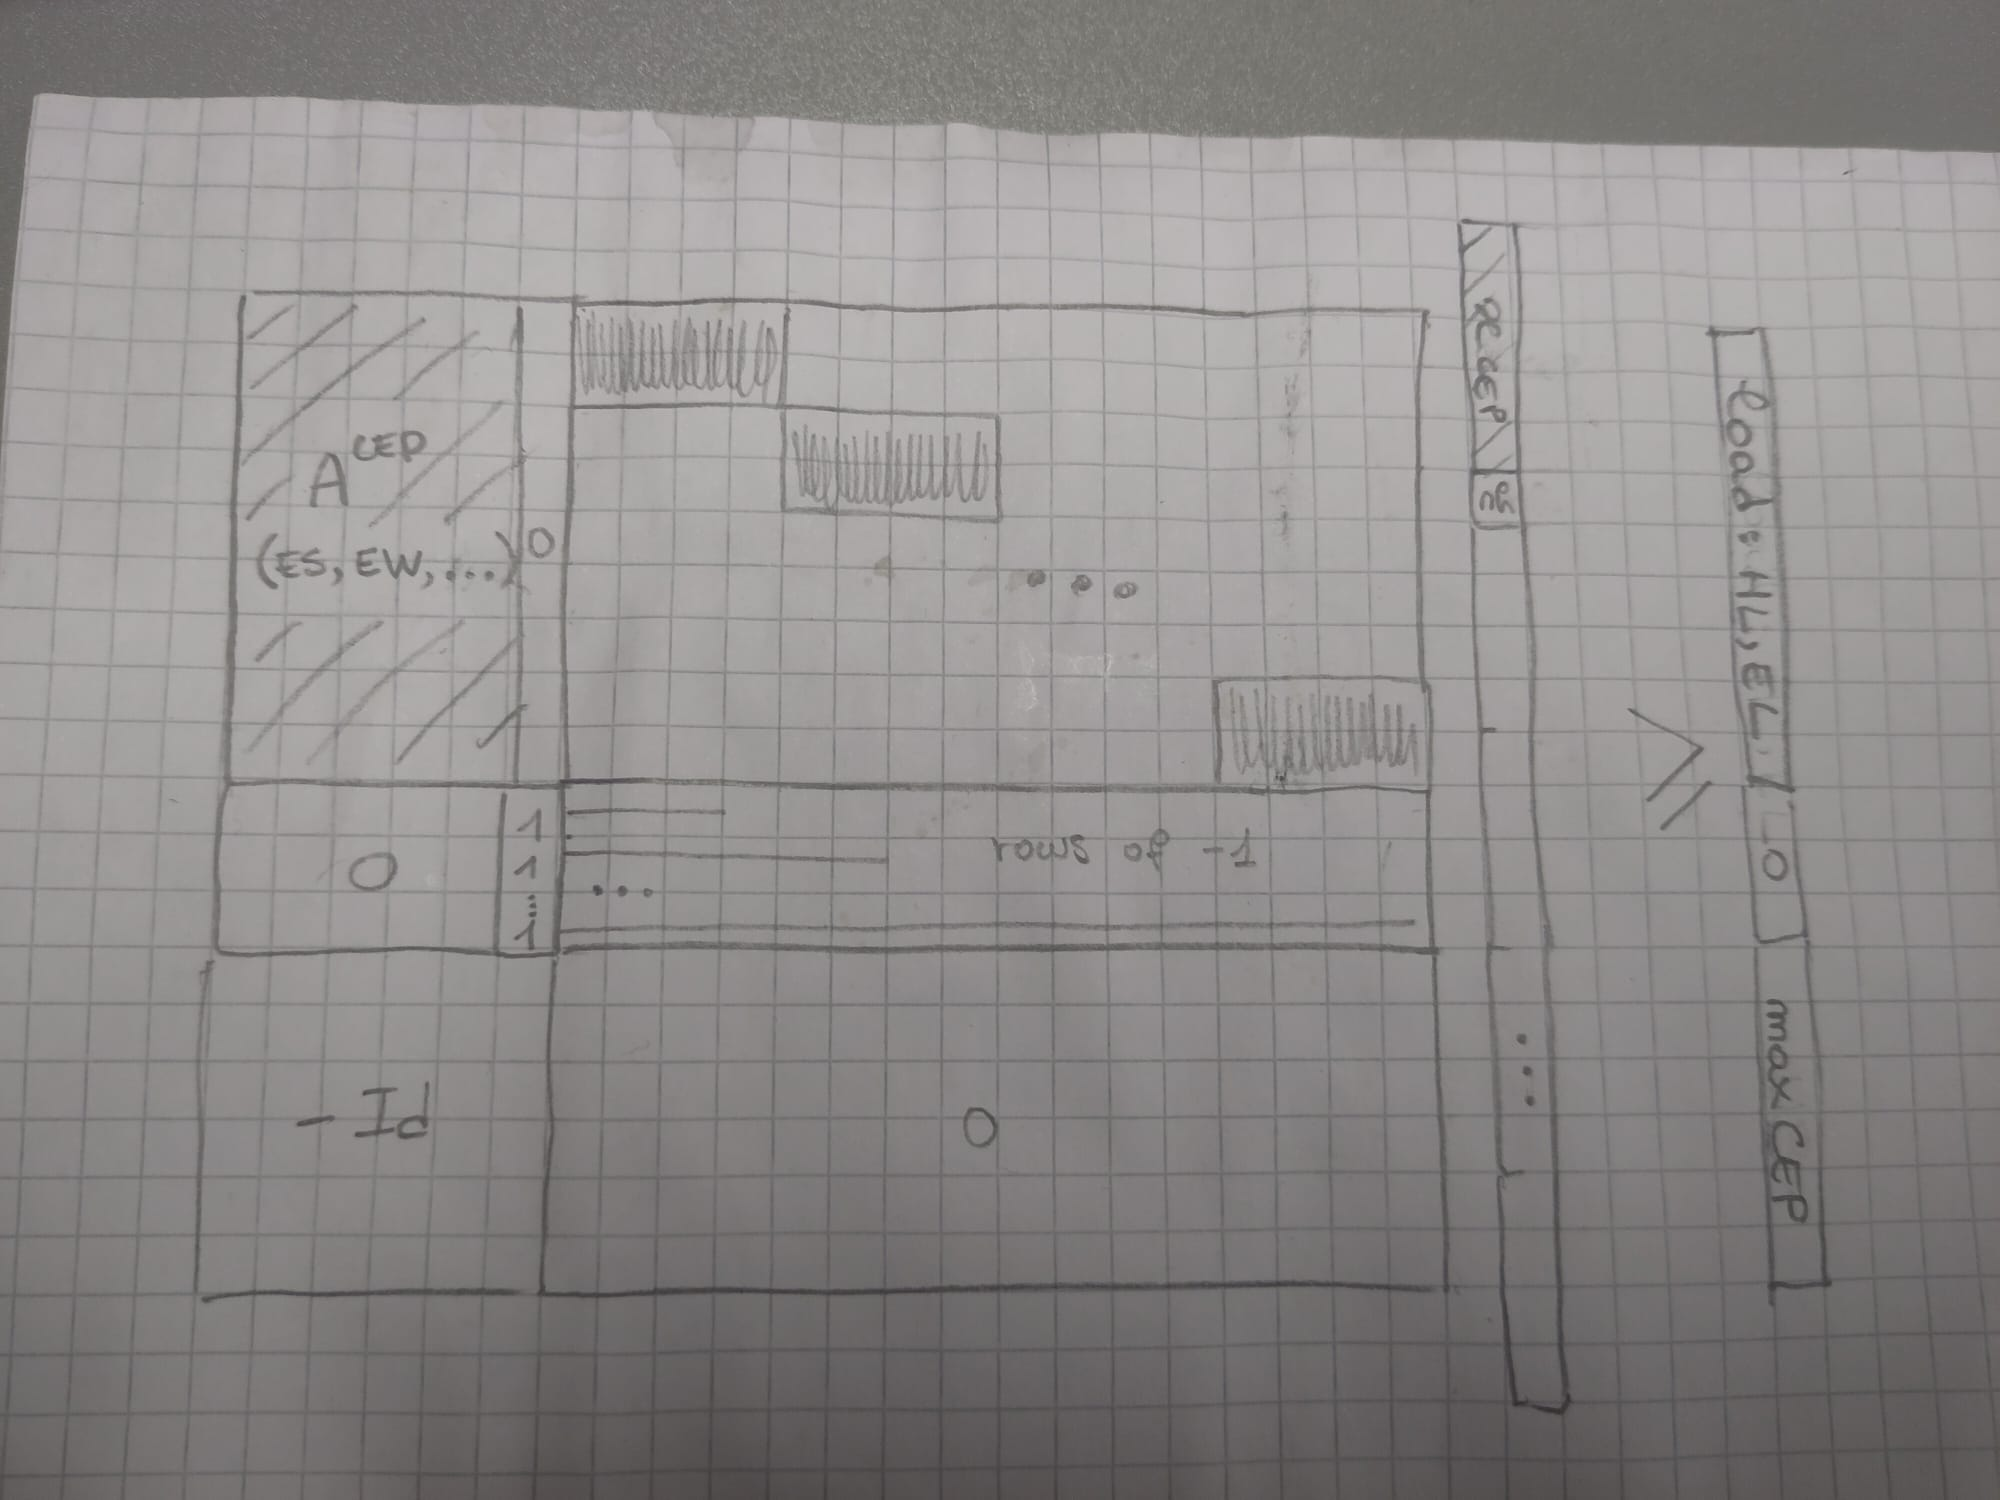
\includegraphics[width=0.75\textwidth]{constraint_matrix.jpeg}
  % figure caption is below the figure
  \caption{To be rendered in LaTeX}
         % Give a unique label
  \end{figure}

 
% For one-column wide figures use
\begin{figure}
  % Use the relevant command to insert your figure file.
  % For example, with the graphicx package use
    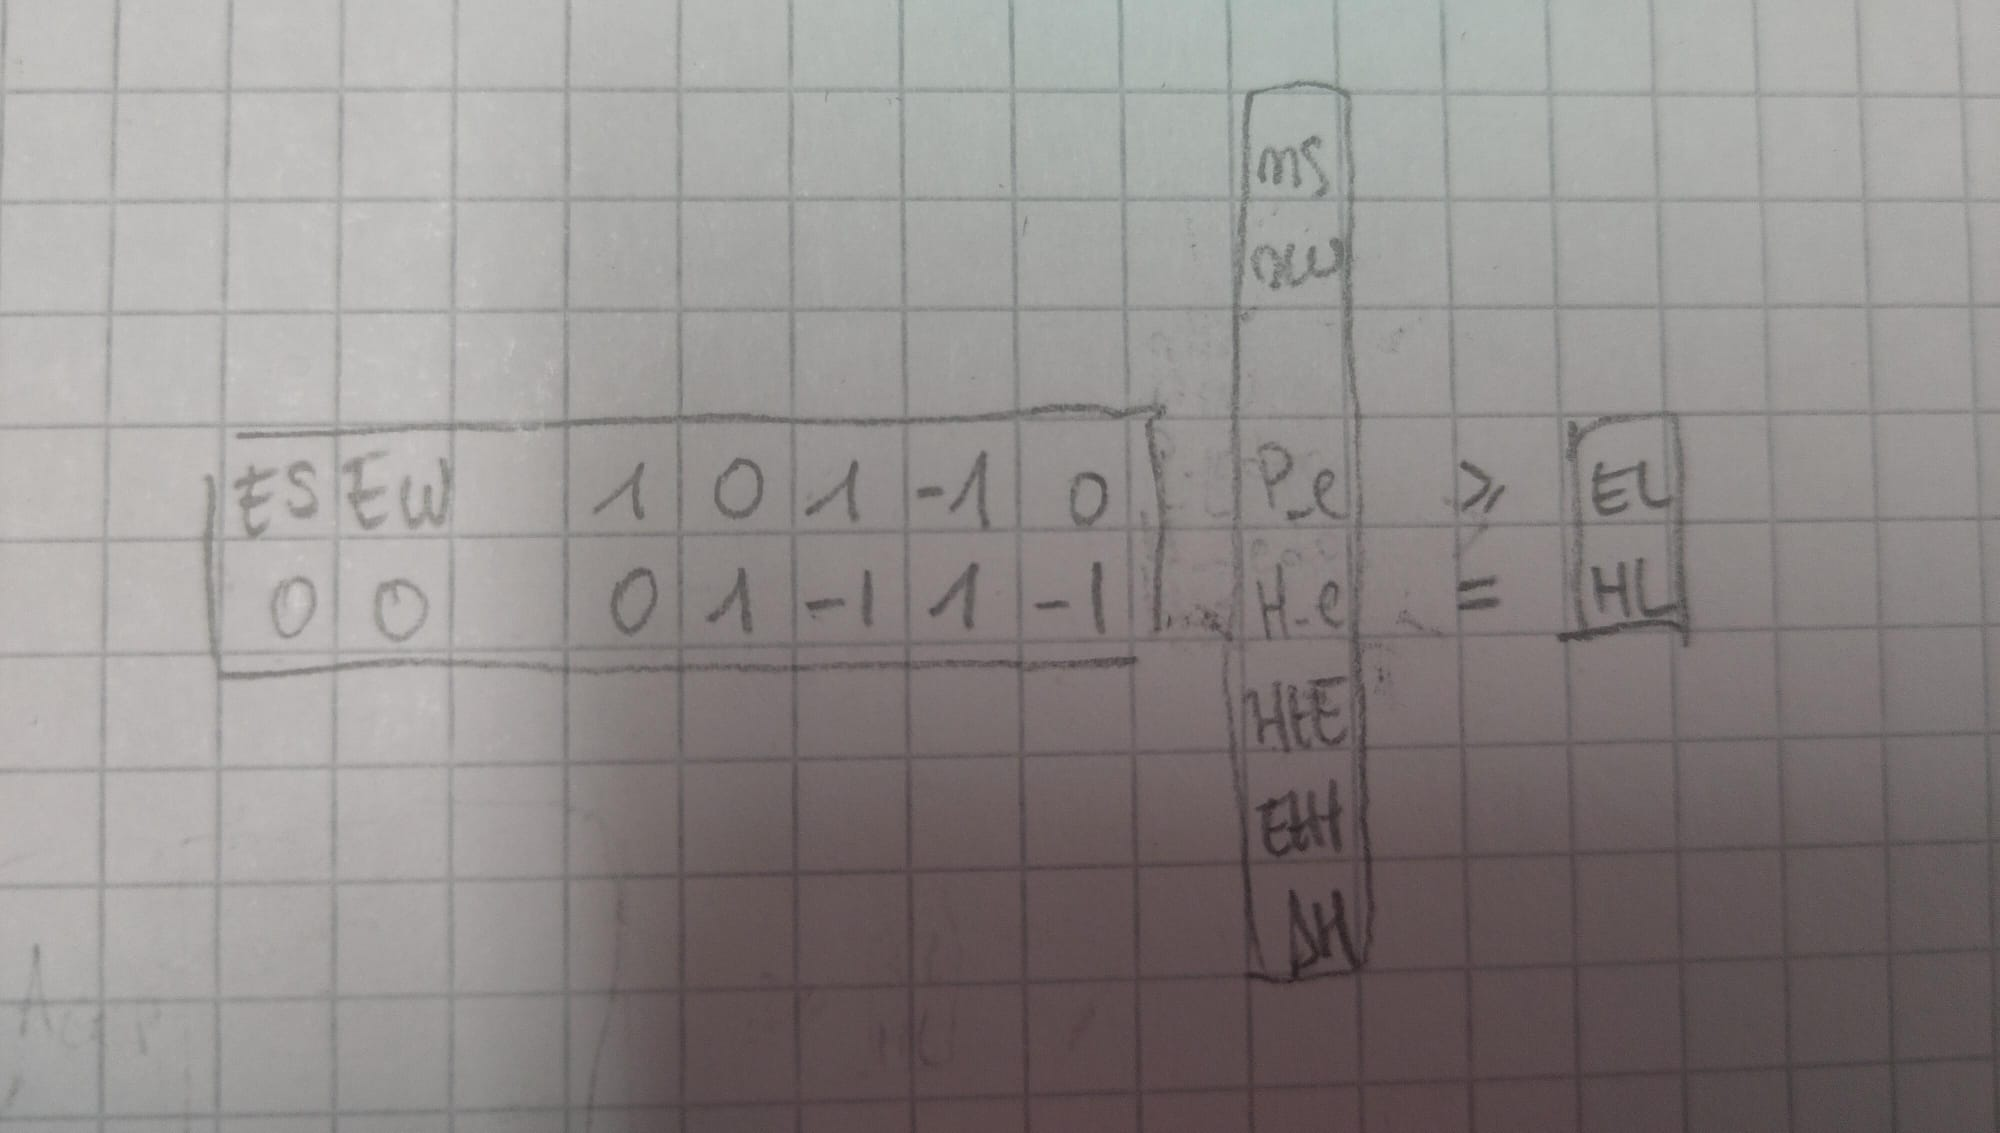
\includegraphics[width=0.75\textwidth]{single_block.jpeg}
  % figure caption is below the figure
  \caption{To be rendered in LaTeX (and correct with coeff 0.033)}
         % Give a unique label
  \end{figure} 








%%%%%%%%%%%%%%%%%%%%%%%%%%%%%%%%%%%%%%%%%%%%%%%%%%%%%%%%%%%%%%%%%%%%%%%%%%%%%%%%%%%%

\subsection{Iteration on time partitions}
\textcolor{red}{idea: aggregated problem is relaxation, so we can solve it (fast) and use it to warm start another solve with some disaggregated interval. How to choose when to disaggregate? We test 3 methods:
\begin{itemize}
\item Random
\item validation function
\item ro - devise a method to "measure" how far an aggregated step is from being allowing extension of the solution to a feasible sol
\end{itemize}
}
\color{gray}
\textbf{While obtaining a feasible solution to \eqref{eq:LP} from \eqref{eq:LPaggr} is not always guaranteed, it is possible under certain assumptions.}
Here, if \(B\) is a matrix having \(I,J\) as set of indexes for the rows and columns respctively, then, for all \(I' \subset I\) and \(J' \subset J\), we denote with \(B_{I',J'}\) the submatrix of \(B\) havins rows in \(I'\) and columns in \(J'\).
\begin{observation}
\label{ob:aggrconstr}
If \((\rowP, \colP)\) is a structure-preserving aggregation, let \(R \in \rowP\) and \(r \in R\). Let \(\tilde{x}\) be a solution to the aggregated problem \eqref{eq:LPaggr}. If \(\tilde{b}_r - \tilde{A}_{R, \colP_{=1}} \tilde{x}_{\colP_{=1}} \neq 0\), define \(\rho_r \coloneqq \frac{b_r - A_{r, \colP_{=1}} \tilde{x}_{\colP_{=1}}}{\tilde{b}_r
 - \tilde{A}_{R, \colP_{=1}} \tilde{x}_{\colP_{=1}}}\). If \(A_{r, \colP_{=1}} = 0\) and \(b_r = 0\), then \(\rho_r\) can be chosen arbitrarily. 

If \(\rho_r \geq 0\) and \(x \in \bR^n\) satisfies \(x_{\colP_{=1}} = \tilde{x}_{\colP_{=1}}\) and \(x_{f^r(C)} = \rho_r \tilde{x}_C\) for all \(C \in \supp(\tilde{A}_R)_{>1}\), then \(x\) satisfies the constraint \(A_r x = b_r\) of the original problem.
\end{observation}

\begin{proof}
From the hypothesis and the definition of structure-preserving aggregation, we have:
\begin{align*}
A_r x &= \sum_{i \in \supp(A_r)} A_{r,i} x_i \\
&= \sum_{S \in \supp(\tilde{A}_R)_{>1}} A_{r,f^r(S)} x_{f^r(S)} + 
\sum_{j \in \colP_{=1}} A_{r,j} x_j \\
&= \sum_{S \in \supp(\tilde{A}_R)_{>1}} \tilde{A}_{R,S} \rho_r \tilde{x}_S + 
\sum_{j \in \colP_{=1}} A_{r,j} x_j
\end{align*}

By the definition of \(\rho_r\):
\begin{align*}
\rho_r \sum_{S \in \supp(\tilde{A}_R)_{>1}} \tilde{A}_{R,S} \tilde{x}_S 
&= \rho_r (\tilde{A}_R \tilde{x} - \tilde{A}_{R,\colP_{=1}} \tilde{x}_{\colP_{=1}}) \\
&= \rho_r (\tilde{b}_R - \tilde{A}_{R,\colP_{=1}} \tilde{x}_{\colP_{=1}}) \\
&= b_r - A_{r, \colP_{=1}} \tilde{x}_{\colP_{=1}}
\end{align*}

Thus, we obtain:
\[
A_r x = b_r
\]
\qed
\end{proof}

A structure-preserving aggregation does not inherently guarantee feasibility for all constraints in the original problem. However, Observation \ref{ob:aggrconstr} illustrates how to partially reconstruct a solution \(x\) for a specific constraint \(r\) by appropriately scaling the aggregated variables within the support of \(A_r\). 

We can now define the hypergraph associated to the aggregation \((\rowP, \colP)\).
\begin{definition}
  The \emph{hypergraph associated to the aggregation \((\rowP, \colP)\)} is the hypergraph \(\cN, \cE\) having as nodes the aggregated variables \(\cN \coloneqq \colP_{>1}\) and as edges the subsest of \(\cN\) that appear together in not row-agnostic constraints.
\end{definition}

When two edges (constraints) in the hypergraph, \(r\) and \(r'\), share aggregated variables, the scaling factors \(\rho_r\) and \(\rho_{r'}\) must be equal to maintain consistency. 
Then if \(\rho_r\) can be defined consistently, by applying observation \ref{ob:aggrconstr}, to all \(r \in R \in \rowP_{>1}\) we can construct a feasible solution for the unaggregated problem \eqref{eq:LPunaggr}. Thus we have: 
\begin{proposition}
\label{prop:xaggfeasible}
If \((\rowP, \colP)\) is a structure-preserving aggregation. Let \(\tilde{x}\) be a solution 
to the aggregated problem \eqref{eq:LPaggr}. If for all \(r \in R \in \rowP_{>1}\) such that  \(\tilde{b}_r - \tilde{A}_{R, \colP_{=1}} \tilde{x}_{\colP_{=1}} = 0\) we have \(A_{r,\colP_{=1}} = 0\) and \(b_r=0\).
Define \(\rho_r \coloneqq \frac{b_r - A_{r, \colP_{=1}} \tilde{x}_{\colP_{=1}}}{\tilde{b}_R - \tilde{A}_{R, \colP_{=1}} \tilde{x}_{\colP_{=1}}}\) for all \(r \in R \in \rowP_{>1}\) such that   \(\tilde{b}_r - \tilde{A}_{R, \colP_{=1}} \tilde{x}_{\colP_{=1}} \neq 0\). If \(\rho_r \geq 0\) and is constant over the connected components of the hypergraph associated to \((\rowP, \colP)\). 
Then \(x_{\colP_{=1}} \coloneqq \tilde{x}_{\colP_{=1}}\) and \(x_{f^r(C)} \coloneqq \rho_r \tilde{x}_C\) for all \(C \in \supp(\tilde{A}_R)\) and \(C \in \colP_{>1}\) is well defined and is feasible solution for the unaggregated problem \eqref{eq:LP}.
\end{proposition}


%\begin{observation}
%  \label{ob:costpreserving}
%  Let \(x\), \(\tilde{x}\) be as defined as in proposition \ref{prop:xaggfeasible}. If \(\rowW_r\tilde{c}_C = c_{f(r,C)}\) for some \(r \in R \in \rowP_{>1}\). Then the cost of \(\tilde{x}\) for the aggregated problem 
%  is equal to the cost of \(x\) in the unaggregated problem. 
%\end{observation}
%\begin{proof}
%  Let \(\tilde{x}\) be a solution to the aggregated problem \eqref{eq:LPaggr}. Using observation \ref{ob:rhoconvex}, for all \(C \in \colP_{>1}\) the cost corresponding to the variable \(\tilde{x}_C\) is 
%  \[
%  \tilde{c}_C\tilde{x}_C = \tilde{c}_C\sum_{r \in R}\rowW_r\rho_r\tilde{x}_C = \sum_{r \in R}\tilde{c}_C\rowW_r\rho_r\tilde{x}_C  = \sum_{r \in R}c_{f(r,C)}x_{f(r,C)}
%  \]
%  Which correspond to the cost of the variables \(\{x_{f(r,C)}\}_{r \in R}\). Thus
%  \[
%  \tilde{c}\tilde{x} = \sum_{C \in \colP_{=1}}\tilde{c}_C\tilde{x}_C + \sum_{C \in \colP_{>1}}\tilde{c}_C\tilde{x}_C = \sum_{C \in \colP_{=1}}c_Cx_C + \sum_{C \in \colP_{>1}}\sum_{r \in R}c_{f(r,C)}x_{f(r,C)} =  \sum_{C \in \colP_{=1}}c_Cx_C + \sum_{j \in \cup_{C \in \colP_{>1}}C}c_{i}x_{i} =  cx
%  \]
%\end{proof}


While row aggregation of a linear problem is a relaxation of the original problem, the same does not apply to column aggregation. However, the column aggregation used for the  Capacity Expansion Problem in this work is still a relaxation. In general a column aggregation of a linear problem is a relaxation of the original problem whenever it is a \emph{constant-coefficients column aggregation}, that is:
\begin{definition}
  A column aggregation  of a linear problem with weights \(\rowW_c,\; c \in C \in \colP \) is a \emph{constant-coefficients column aggregation}  if for all \(c \in C \in \colP\) for all rows \(r \in [m]\), we have \(\rowW_cA_{r,c} = \frac{1}{|C|}\) or  \(\rowW_cA_{r,c} = 0\).  
\end{definition}

That is if for every set \( C \in \rowP \) of variables that are aggregated together, each variable in \( C \) has the same coefficients in every row of the aggregated problem defined by \( \rowP \) and the coefficient is equal to the aggregation weight of the corresponding variable, except for those rows where all the coefficients of the variables are zero.
We then substitute the columns corresponding to \( C \) with a vector containing one in every row in which the coefficients in \(C\) are non zero, otherwise we substitute with zero.

\begin{proposition}
If \((\rowP,\colP)\) is a structure-preserving, constant-coefficients column aggregation,
if the hypothesis of proposition \ref{prop:xaggfeasible} holds then the aggregated problem \eqref{eq:LPaggr} is exact and \(x\) is an optimal solution.
\end{proposition}

\begin{proof}
  Since for observation \ref{ob:costpreserving}, the cost of the aggregated problem is equal to the cost of \(x\) in the unaggregated problem, we only need to show that the aggregated problem is a relaxation of the unaggregated problem.
  Let \(x\) be a solution to the unaggregated problem \eqref{eq:LP}. For all \(C \in \colP_{=1}\) let \(\tilde{x}_C \coloneqq x_C\).
  Since  \(\{f^r(C)\}_{r \in \cup_{R\in \rowP_{>1}}, C \in \colP} = \cup_{C \in \colP_{>1}}C\), for all \(c \in C \in \colP_{>1}\), exists \(r \in R \in \rowP_{>1}\) and \(C \in \colP_{>1}\) such that \(f^r(C) = c\).
  Then let \(\tilde{x}_C \coloneqq \sum_{c \in C}A_{r,c}x_c\). Since if \(f^{r}(C)= f^{r'}(C')\) implies that \(C=C'\), \(x\) is well defined.
  Lastly for all \(R \in \rowP\) we have:
  \[\tilde{A}_R\tilde{x} = \sum_{r \in R} \left( \sum_{C \in \colP_{=1}}\rowW_rA_{r,c}\tilde{x}_C + \sum_{C\in \supp(\tilde{A}_r)_{>1}} \tilde{x}_C \right) = \sum_{r \in R} \left( \sum_{C \in \colP_{=1}}\rowW_rA_{r,c}x_C + \sum_{C\in \supp(\tilde{A}_r)_{>1}} \sum_{c \in C}A_{r,c}x_c \right) = \sum_{r \in R} \tilde{\rho_r} b_r = \tilde{b}_R 
  \]
  \qed
\end{proof}


\subsection{Application to Capacity Expansion Problem}

We now apply the results of the previous section to the Capacity Expansion Problem. 
%\textcolor{violet}{
%TODO:
%\begin{itemize}
%  \item What are the connected components of the hypergraph as defined in the previous sectors? each connected component looks like the hypergraph of the ED at a fixed timestep. Why can we not consider the edges corresponding to hydrogen storage? because however \(\rho\)s are chosen, they hold, so they don't force \(\rho\) to be equal over the nodes it connects.
%  \item What does it mean? Given an aggregated problem, we are interested in which time intervals are problematic, since the ones which have well define \(\rho\) could be disgragated and obtain the same solution, we disgragate the ones in which the \(\rho\)s are far from being well defines, that is we have two constraints in the same connected components with really different \(\rho_r\).
%  \item What is \(\rho_r\), since the aggregated variables are only second stage variables. Let's consider \(\rho_r\) with \(r \in R\), and let \(t_r\) and \(n \in \cN\) be respectively the time step and the node corresponding to the constraint \(r\).Let the net energy production at time \(t\) in \(n\): that is demand in \(n\) minus any renewable power produced in \(n\). Then \(\rho_r\) corresponds to fraction between the net energy production at time \(t\) and the net energy production during the interval \(T\) with \(t \in T\).
%  \item How to disaggregate: Thus we calculate \(\rho_(n,t)\) for all nodes in the network and al timestep, and disagregate thos with highest variance for fixed \(t\). (since, fixed t the should all be equal for the solution be feasible for the problem obtained by disagregating the time interval T). \\
%  \item How much to disaggregate: One could either subdivide each time interval into finer time intervals, or to the single timesteps. For the former, one could keep the intervals in which the variance of \(\rho_r\) is small, together, and divide in single timesteps the rest.
%  \item Initial aggregation: to calculate \(\rho_r\) we need to have solved already an aggregated problem, so it's not too insightful. But we can start by grouping together intervals by putting "peaks" on the extremes, that is peak of demand and production, and then subdividing equally the so obtained intervals.
%  \item Write well how to calculate \(\rho_r\)
%\end{itemize}
%}

\color{violet}


It can be easily checked that:

\begin{observation}
  The aggregation of the Capacity Expansion Problem (CEP) is a structure-preserving aggregation with constant coefficients. Furthermore, the constraints \eqref{eq:delta_hydrogen_constraints} are \(\rho\)-agnostic.
\end{observation}

Since the only constraints linking variables across different time steps are those in \eqref{eq:delta_hydrogen_constraints}, the connected components of the hypergraph representing the aggregation correspond to the hypergraphs of the Energy Dispatch (ED) at each time step. Specifically, there is one connected component per time step, with nodes representing the variables at that step. To construct a feasible solution from the aggregated problem, it is sufficient for \(\rho_r\) to be constant across constraints within the same time step.

Using the definition of \(\rho_r\), it can be shown that for each time step \(t \in T \in \cT\), this corresponds to the ratio between the net energy production at time \(t\) and the net energy production over the interval \(T\). Hence, the conditions of Proposition \ref{prop:xaggfeasible} are met if, for a fixed time step \(t\), this ratio is the same for all nodes in the network, and if, during the interval \(T\), the net production at each node is consistently positive or consistently negative. Thus, we state:

\begin{observation}
  \label{obs:cep_agg_feasible}
  If for each time step \(t \in T \in \cT\), the ratio of the net energy production at time \(t\) to the net energy production over the interval \(T\) is the same for all nodes in the network, and if, throughout the interval \(T\), the net production at each node is either always positive or always negative, then the aggregated problem is exact.
\end{observation}

Although this is not generally the case, it suggests an iterative procedure for refining the solution of the aggregated problem. At each iteration, we refine the time partition of the aggregated problem, selecting the time interval to be refined based on the extent to which it violates the conditions of Observation \ref{obs:cep_agg_feasible}. Specifically, we split intervals where the net production changes sign, and those intervals \(T\) in which, for a fixed time step \(t \in T\), the ratio between the net energy production at time \(t\) and the net energy production over the interval \(T\) exhibits the largest variance.


%%%%%%%%%%%%%%%%%%%%%%%%%%%%%%%%%%%%%%%%%%%%%%%%%%%%%%%%%%%%%%%%%%%%%%%%%%%%%%%%%%%%%%%%%%%%%%%%%%%%


\section{COMPUTATIONAL RESULTS}
\color{gray}
To test the methods described in this paper, we consider a simple 5-node network over a one-year period with timesteps of 1 hour. In this section, we compare the following methods for iterating on the aggregated problem: (1) randomly selecting the interval to refine, (2) selecting the interval with the highest \(\rho\)-variance as defined in Section \ref{}, or (3) selecting the interval where the validation function \ref{} fails.
The scenarios are generated as described in Section \ref{subsec:scenarios} in the Appendix. The computational tests were carried out on an Intel(R) Core(TM) i7-13700H CPU @ 2.40GHz with 16 GB RAM.

INSERT PLOT COMPARING RHO-Random
INSERT PLOT COMPARING RHO-FUNCTION


% \subsection{SINGLE NODE NETWORK}
% First, an electrical grid with a single node is considered (corresponding ideally to an area with uniform
% weather conditions, highly connected at low cost). A first section will consider realistic parameter
% combinations and describe the results given by the solver, conducting a parameter sensitivity analysis. A
% second section will describe a validation function that checks the results of the capacity expansion
% problem for feasibility on new scenarios. Concurrently, a cost function is designed to give more realistic
% cost estimates compared to the optimal value given by the solver.

% Results are computed for a multiple node network, with additional edge variables and parameters. When
% considering a network with more than a single node, computational costs increase rapidly. Thus in the
% first section, a small analysis is carried out to determine acceptable time steps on which time dependent
% data can be aggregated (the gathered data is usually on hourly steps) while maintaining the quality of the
% solution. Some examples are then considered, and the network dynamics that arise with the introduction
% of edge variables are described. A mixed approach is then used to design a validation function that can
% deal with the complexity arising from the introduction of the network structure in the model.


\section{CONCLUSION}





\color{black}

\section{APPENDIX}

\subsection{SCENARIO GENERATION}\label{generation}

To estimate the optimal capacities for the CEP through a stochastic approach, realistic and diverse weather scenarios are needed, so to capture the variability and uncertainty of power generation through renewable sources over extended periods. 
In order to generate such scenarios, samples are extracted from a joint probability density function (PDF) fit on historical data. \textcolor{pink}{In the following subsection,} we use \(Y_t\) to denote the stochastic process of generated power observations for either solar or wind in a single country.
In our project, we used an hourly time step (T=\{1...8760\}) and fit the wind and solar distributions separately for each country considered.
To model the marginal probability distributions corresponding to the power output of wind turbines for each hour of the year, a Weibull distribution was used, justified by its proven effectiveness in capturing the variability and skewness of wind power distributions \textcolor{green}{\cite{weibullwind}}. 
For solar power, Beta distributions were employed, as in \textcolor{green}{\cite{betaPV}}. \\
\indent  To fit our model, we used a dataset containing 30 years of data for various European countries, which was collected by \textcolor{green}{\cite{30y_gen}}. 
On the other hand, electricity load is taken from the \textcolor{green}{\href{https://www.entsoe.eu/data/power-stats/}{ENTSO-E Statistical Reports}}. \textcolor{red}{explain how is HL obtained}
\textcolor{pink}{In this simple model, while fitting on historical data we did not account for possible changes in future climate, since the focus lies mostly in the computational aspect.}\\
To account for interdependence between temporally near time steps, we coupled these distributions using a Gaussian Copula approach, which captures the dependencies between hourly power outputs effectively. \textcolor{pink}{This approach accurately mimics common weather phenomena: The Gaussian Copula represents well the coupled behavior in renewable stochastic systems} \textcolor{green}{\cite{GaussCopula}}. \\
\indent A possible improvement of the generation process could be to fit wind and PV data jointly in the copula step, potentially also including load scenarios with the generation scenarios through the same approach. This would consider dependence between Energy Demand and weather conditions, but it would necessitate of the historical dataset provided for the corresponding grid, and would also further increase computational costs.


%\subsubsection{Stochastic Processes description}
%The stochastic processes of power observations will be denoted as \(Y_t\). Where \(t \in T\), is the set indexing all the random variables which want to be considered jointly.
%We assume that the random variable \(Y_t\) has either a Weibull distribution, in the case of Wind Power, or a Beta distribution in the case of Solar Power. 

\subsubsection{Parametric Estimation of Wind Power distribution}\label{subsection: weib estim}

The parameters defining the Weibull Distribution are estimated using the Maximum Likelyhood Estimation (MLE). The Weibull density function is given by:
\[
f(x; \theta, \gamma) = \left(\frac{\gamma}{\theta}\right)x^{\gamma-1}\exp\left(-\left(\frac{x}{\theta}\right)^\gamma\right)
\]

where \(\theta, \gamma > 0\) are the scale and shape parameters, respectively. Given observations \(X_1, \ldots, X_n\), the log-likelihood function is:

\[
\log L(\theta, \gamma) = \sum_{i=1}^n \log f(X_i \mid \theta, \gamma)
\]

The optimum solution is found by searching for the parameters for which the gradient is zero :

\begin{equation}
\frac{\partial \log L}{\partial \theta} = -\frac{n \gamma}{\theta} + \frac{\gamma}{\theta^2} \sum_{i=1}^{n} x_i^\gamma = 0
\end{equation}

Eliminating $\theta$, we get:

\begin{equation}
\left[ \frac{\sum_{i=1}^{n} x_i^\gamma \log x_i}{\sum_{i=1}^{n} x_i^\gamma} - \frac{1}{\gamma} \right] = \frac{1}{n} \sum_{i=1}^{n} \log x_i
\end{equation}

This can be solved to get the MLE estimate $\hat{\gamma}$. \textcolor{pink}{This can be accomplished with the aid of standard iterative procedures such as the Newton-Raphson method or other numerical procedures. This is done with the aid of the package \emph{scipy}.} Once $\hat{\gamma}$ is found, $\hat{\theta}$ can be determined in terms of $\hat{\gamma}$ as:

\begin{equation}
\hat{\theta} = \left( \frac{1}{n} \sum_{i=1}^{n} x_i^{\hat{\gamma}} \right)^{\frac{1}{\hat{\gamma}}}
\end{equation}



%%%%%%%%%%%%%%%%%%%%%%%%%%%%%%%%%%%%%%%%%%%%%%%%%%%%%%%%%%%%%%%%%%%%%%%%%%%

\subsubsection{Parametric Estimation of Solar Power distribution}
\label{subsection: beta estim}

To estimate the \(\alpha\) and \(\beta\) parameters defining the Beta distribution \(Y\), we use the Method of Moments.
The mean of the random variable \(Y\) can be expressed as \(\E\left[ Y\right] = \frac{\alpha}{\alpha + \beta} \) and the variance as \(\var [Y]= \frac{\alpha + \beta}{(\alpha + \beta)(\alpha + \beta + 1)}\). In particular by explicating \(\beta\) in the first equation and substituting it in the second equation we obtain that:
\begin{equation}
\begin{cases}
\alpha = \mathbb{E}[X] \left( \frac{\mathbb{E}[X](1 - \mathbb{E}[X])}{\mathrm{Var}[X]} - 1 \right) \\
\beta = (1 - \mathbb{E}[X]) \left( \frac{\mathbb{E}[X](1 - \mathbb{E}[X])}{\mathrm{Var}[X]} - 1 \right)
\end{cases}
\end{equation}
By substituting the mean and the variance with their empirical approximation we obtain the Method of Moments estimator for \(\alpha\) and \(\beta\).

%%%%%%%%%%%%%%%%%%%%%%%%%%%%%%%%%%%%%%%%%%%%%%%%%%%%%%%%%%%%%%%%%%%%%%%%%%%

\subsubsection{Parametric Copula Estimation}
The cumulative density function of both the Weibull and Beta distributions are continuous and invertible. Therefore, the random variables \( U_t \coloneqq F_{Y_t}(Y_t) \) have a uniform distribution over \([0,1]\). The copula of the random variables \(\{Y_t\}_{t \in T}\) is defined as the function \(C: [0,1]^T \to [0,1]\) such that 
\begin{equation}
C(F_{Y_1}(y_1), \ldots, F_{Y_T}(y_{|T|})) = P(Y_1 \leq y_1, \ldots, Y_{|T|} \leq y_{|T|}).
\end{equation}
This function always exists because of Sklar's Theorem \textcolor{green}{cite Sklar?}. For a given correlation matrix \(\Sigma\), the Gaussian Copula with parameter matrix \(\Sigma\) is defined as 
\[\CG(u_1,\ldots,u_{T}) \coloneqq \Phi_{\Sigma}(\Phi^{-1}(u_1),\ldots, \Phi^{-1}(u_T)),\] 
where \(\Phi,\; \Phi_{\Sigma}\) are the cumulative distribution functions of Gaussian variables having distribution \(\mathcal{N}(0,1)\) and \( \mathcal{N}(\mathbf{0},\Sigma)\) respectively. 
In particular if \(\CG\) is the copula associated with the random variables \(\{Y_t\}_{t \in T}\) then we have that the random variables \(Z_t = \Phi^{-1}(F_{Y_t}(Y_t)) = \Phi^{-1}(U_t)\) have joint distribution equal to \(\mathcal{N}(0, \Sigma)\). This follows from: \\
\begin{align*}
P(Z_1 \leq z_1, \ldots, Z_T \leq z_t) &= P(\Phi^{-1}(U_1) \leq z_1, \ldots, \Phi^{-1}(U_T) \leq z_T) = \\
&= P(U_1 \leq \Phi(z_1), \ldots, U_T \leq \Phi(z_T)) = \\
&= \CG(\Phi(z_1), \ldots, \Phi(z_t)) =  \\
&= \Phi_{\Sigma}(z_1, \ldots, z_T)
\end{align*}
In particular, given the realization \(\{y_{t,j}\}_{t \in t, j \in J}\) of the variables \(\{Y_t\}_{t \in T}\), an unbiased estimation of the parameter matrix \(\Sigma\) is the empirical covariance matrix \(\hat \Sigma\) of the samples \(\{\Phi^{-1}(\hat{F}_{Y_t}(y_{t,j}))\}_{t\in T, j \in J}\), where \(\hat{F}_{Y_t}\) is the estimated marginal distribution of the variable \(Y_t\) \textcolor{green}{as seen in subsection \ref{subsection: weib estim} and subsection \ref{subsection: beta estim}}.\\


Finally, we can generate samples from a Multivariate Gaussian random variable \((Z_{t}, t \in T)\) having distribution \(\mathcal{N}(0, \hat \Sigma)\).  Then the power output scenarios are obtained from these samples by following the previous steps backwards, that is, for each sample, computing \(\hat F_{t}^{-1}(\Phi(Z_{t}))\) for all \(t\in T\). \\

%%%%%%%%%%%%%%%%%%%%%%%%%%%%%%%%%%%%%%%%%%%%%%%%%%%%%%%%%%%%%%%%%%%%%%%%%%%


%\begin{acknowledgements}
%If you'd like to thank anyone, place your comments here
%and remove the percent signs.
%\end{acknowledgements}


% Authors must disclose all relationships or interests that 
% could have direct or potential influence or impart bias on 
% the work: 
%
% \section*{Conflict of interest}
%
% The authors declare that they have no conflict of interest.


% BibTeX users please use one of
%bibliographystyle{spbasic}      % basic style, author-year citations
%\bibliographystyle{spmpsci}      % mathematics and physical sciences
%\bibliographystyle{spphys}       % APS-like style for physics
%\bibliography{sample}   % name your BibTeX data base

%\printbibliography[
%heading=bibintoc,
%title={Bibliography}]

% % Non-BibTeX users please use
\begin{thebibliography}{}
% %
% % and use \bibitem to create references. Consult the Instructions
% % for authors for reference list style.
% %
% \bibitem{RefJ}
% % Format for Journal Reference
% Author, Article title, Journal, Volume, page numbers (year)
% % Format for books
% \bibitem{RefB}
% Author, Book title, page numbers. Publisher, place (year)
% % etc

\bibitem{review_math_opt}
Michal Jasinski, Arsalan Najafi, et al,
Operation and Planning of Energy Hubs Under Uncertainty - A Review of Mathematical Optimization Approaches,
2022


\bibitem{European_H2_Market_landscape}
Author, European Hydrogen Market Landscape - November 2023 Report, page numbers. Publisher, place (year)


\bibitem{30y_gen}
Stefan Pfenninger and Iain Staffell. “Long-term patterns of European PV output us-
ing 30 years of validated hourly reanalysis and satellite data”. In: Energy 114 (2016),
pp. 1251–1265. issn: 0360-5442. doi: https://doi.org/10.1016/j.energy.2016.08.
060.

\bibitem{Gurobi}
Gurobi Optimization, LLC: Gurobi Optimizer Reference Manual (2024). https://www.gurobi.com

\bibitem{deterministic}
M. Hashem Nehrir, Power Management of a Stand-Alone Wind/Photovoltaic/Fuel Cell Energy System, IEEE Transactions on Energy Conversion, 2008. DOI: 10.1109/TEC.2007.914200

% %@article{European_H2_Market_landscape,
% %title = {European Hydrogen Market Landscape - November 2023 Report},
% % journal = {European Journal of Operational Research},
% % volume = {},
% % number = {1},
% % pages = {},
% % year = {2023},
% % doi = {},
% % url = {https://observatory.clean-hydrogen.europa.eu/sites/default/files/2023-11/Report%2001%20-%20November%202023%20-%20The%20European%20hydrogen%20market%20landscape.pdf},
% % author = {European Hydrogen Observatory},
% % keywords = {},
% % abstract = {}
% % }

% \bibitem{WindDataSet}
% Author, Book Title, page numbers. Publisher, place (year)

% % @article{WindDataSet,
% % title = {Using bias-corrected reanalysis to simulate current and future wind power output},
% % journal = {Energy},
% % volume = {114},
% % pages = {1224-1239},
% % year = {2016},
% % issn = {0360-5442},
% % doi = {https://doi.org/10.1016/j.energy.2016.08.068},
% % url = {https://www.sciencedirect.com/science/article/pii/S0360544216311811},
% % author = {Iain Staffell and Stefan Pfenninger},
% % keywords = {Wind power, Wind farm, Reanalysis, Capacity factor, Energy yield, Europe},
% % abstract = {Reanalysis models are rapidly gaining popularity for simulating wind power output due to their convenience and global coverage. However, they should only be relied upon once thoroughly proven. This paper reports the first international validation of reanalysis for wind energy, testing NASA's MERRA and MERRA-2 in 23 European countries. Both reanalyses suffer significant spatial bias, overestimating wind output by 50% in northwest Europe and underestimating by 30% in the Mediterranean. We derive national correction factors, and show that after calibration national hourly output can be modelled with R2 above 0.95. Our underlying data are made freely available to aid future research. We then assess Europe's wind resources with twenty-year simulations of the current and potential future fleets. Europe's current average capacity factor is 24.2%, with countries ranging from 19.5% (Germany) to 32.4% (Britain). Capacity factors are rising due to improving technology and locations; for example, Britain's wind fleet is now 23% more productive than in 2005. Based on the current planning pipeline, we estimate Europe's average capacity factor could increase by nearly a third to 31.3%. Countries with large stakes in the North Sea will see significant gains, with Britain's average capacity factor rising to 39.4% and Germany's to 29.1%.}
% % }


% \bibitem{PVDataSet}
% Author, Book Title, page numbers. Publisher, place (year)
% % @article{PVDataSet,
% % title = {Long-term patterns of European PV output using 30 years of validated hourly reanalysis and satellite data},
% % journal = {Energy},
% % volume = {114},
% % pages = {1251-1265},
% % year = {2016},
% % issn = {0360-5442},
% % doi = {https://doi.org/10.1016/j.energy.2016.08.060},
% % url = {https://www.sciencedirect.com/science/article/pii/S0360544216311744},
% % author = {Stefan Pfenninger and Iain Staffell},
% % keywords = {Solar energy, Meteorological reanalysis, Satellite irradiance estimation, Renewables, Grid integration of renewables},
% % abstract = {Solar PV is rapidly growing globally, creating difficult questions around how to efficiently integrate it into national electricity grids. Its time-varying power output is difficult to model credibly because it depends on complex and variable weather systems, leading to difficulty in understanding its potential and limitations. We demonstrate how the MERRA and MERRA-2 global meteorological reanalyses as well as the Meteosat-based CM-SAF SARAH satellite dataset can be used to produce hourly PV simulations across Europe. To validate these simulations, we gather metered time series from more than 1000 PV systems as well as national aggregate output reported by transmission network operators. We find slightly better accuracy from satellite data, but greater stability from reanalysis data. We correct for systematic bias by matching our simulations to the mean bias in modeling individual sites, then examine the long-term patterns, variability and correlation with power demand across Europe, using thirty years of simulated outputs. The results quantify how the increasing deployment of PV substantially changes net power demand and affects system adequacy and ramping requirements, with heterogeneous impacts across different European countries. The simulation code and the hourly simulations for all European countries are available freely via an interactive web platform, www.renewables.ninja.}
% % }


% \bibitem{Dunkelflaut}
% Author, Book Title, page numbers. Publisher, place (year)
% % @Article{Dunkelflaut,
% % AUTHOR = {Li, Bowen and Basu, Sukanta and Watson, Simon J. and Russchenberg, Herman W. J.},
% % TITLE = {A Brief Climatology of Dunkelflaute Events over and Surrounding the North and Baltic Sea Areas},
% % JOURNAL = {Energies},
% % VOLUME = {14},
% % YEAR = {2021},
% % NUMBER = {20},
% % ARTICLE-NUMBER = {6508},
% % URL = {https://www.mdpi.com/1996-1073/14/20/6508},
% % ISSN = {1996-1073},
% % DOI = {10.3390/en14206508}
% % }



% \bibitem{betaPV}
% Author, Book Title, page numbers. Publisher, place (year)
% % @article{betaPV,
% % title = {Prediction interval of wind power using parameter optimized Beta distribution based LSTM model},
% % journal = {Applied Soft Computing},
% % volume = {82},
% % pages = {105550},
% % year = {2019},
% % issn = {1568-4946},
% % doi = {https://doi.org/10.1016/j.asoc.2019.105550},
% % url = {https://www.sciencedirect.com/science/article/pii/S1568494619303308},
% % author = {Xiaohui Yuan and Chen Chen and Min Jiang and Yanbin Yuan},
% % keywords = {Wind power, Prediction interval, Long short-term memory neural network, Beta distribution, Particle swarm optimization},
% % abstract = {Prediction interval of wind power (PIWP) is crucial to assessing the economic and safe operation of the wind turbine and providing support for analysis of the stability of power systems. The hybrid model (Beta-PSO-LSTM) of long short-term memory (LSTM) neural network and Beta distribution function based particle swarm optimization (PSO) is put forward for prediction interval of wind power. In order to enhance the performance of the Beta-PSO-LSTM for PIWP in training process, wind power series are divided into different power intervals, and then the Beta-PSO-LSTM is used to estimate each power interval of the original wind power series. Furthermore, based on the analysis of the interval forecasting error information in wind power training data set, Beta distribution model is proposed to get better PIWP, and PSO is used to optimize the parameters of the model. Finally, the proposed Beta-PSO-LSTM model is compared with the Beta distribution optimized by PSO based the BP neural network (Beta-PSO-BP), the normal distribution based LSTM neural network (Norm-LSTM), Beta distribution based LSTM neural network (Beta-LSTM), and Beta distribution optimized by iterative method based LSTM neural network (Beta-IM-LSTM) for PIWP. The simulation results show that the PIWP obtained by the Beta-PSO-LSTM model has higher reliability and narrower interval bandwidth, which can provide decision support for the safe and stable operation of power systems.}
% % }


% \bibitem{GaussCopula}
% Author, Book Title, page numbers. Publisher, place (year)
% % @ARTICLE{GaussCoupula,
% %   author={Papaefthymiou, George and Kurowicka, Dorota},
% %   journal={IEEE Transactions on Power Systems}, 
% %   title={Using Copulas for Modeling Stochastic Dependence in Power System Uncertainty Analysis}, 
% %   year={2009},
% %   volume={24},
% %   number={1},
% %   pages={40-49},
% %   keywords={Power system modeling;Stochastic systems;Power system analysis computing;Uncertainty;Random variables;Power system planning;Stochastic processes;Power generation;Context modeling;Aggregates;Copula;correlation;Monte Carlo simulation;stochastic dependence;stochastic generation;uncertainty analysis;wind power},
% %   doi={10.1109/TPWRS.2008.2004728}}


% \bibitem{weibullwind}
% Author, Book Title, page numbers. Publisher, place (year)
% % @article{weibullwind,
% % title = {Evaluation of wind power production prospective and Weibull parameter estimation methods for Babaurband, Sindh Pakistan},
% % journal = {Energy Conversion and Management},
% % volume = {78},
% % pages = {956-967},
% % year = {2014},
% % issn = {0196-8904},
% % doi = {https://doi.org/10.1016/j.enconman.2013.06.062},
% % url = {https://www.sciencedirect.com/science/article/pii/S019689041300589X},
% % author = {Shahnawaz Farhan Khahro and Kavita Tabbassum and Amir Mahmood Soomro and Lei Dong and Xiaozhong Liao},
% % keywords = {Wind energy, Power density function, Weibull distribution, Frequency distribution, Wind rose},
% % abstract = {Pakistan is currently experiencing an acute shortage of energy and urgently needs new sources of affordable energy that could alleviate the misery of the energy starved masses. At present the government is increasing not only the conventional energy sources like hydel and thermal but also focusing on the immense potential of renewable energy sources like; solar, wind, biogas, waste-to-energy etc. The recent economic crisis worldwide, global warming and climate change have also emphasized the need for utilizing economic feasible energy sources having lowest carbon emissions. Wind energy, with its sustainability and low environmental impact, is highly prominent. The aim of this paper is to explore the wind power production prospective of one of the sites in south region of Pakistan. It is worth mentioning here that this type of detailed analysis is hardly done for any location in Pakistan. Wind power densities and frequency distributions of wind speed at four different altitudes along with estimated wind power expected to be generated through commercial wind turbines is calculated. Analysis and comparison of 5 numerical methods is presented in this paper to determine the Weibull scale and shape parameters for the available wind data. The yearly mean wind speed of the considered site is 6.712m/s and has power density of 310W/m2 at 80m height with high power density during April to August (highest in May with wind speed 9.595m/s and power density 732W/m2). Economic evaluation, to exemplify feasibility of installing wind turbines, is also done. The estimated cost of per kWh of electricity from wind is calculated as 0.0263US$/kWh. Thus the candidate site is recommended for some small stand-alone systems as well as for wind farm.}
% % }


% \bibitem{future_climate}
% Author, Book Title, page numbers. Publisher, place (year)
% % @article{future_climate,
% %     author = {Bett, P. E., Thornton, H. E., and Clark, R. T.},
% %     title = {European wind variability over 140 yr},
% %     journal = {Adv. Sci. Res., 10, 51–58},
% %     year = {2013}
% % }




\end{thebibliography}

\end{document}
% end of file template.tex

